\documentclass[10pt]{memoir}
\setstocksize{220mm}{155mm} 	        
\settrimmedsize{220mm}{155mm}{*}	
\settypeblocksize{170mm}{116mm}{*}	
\setlrmargins{18mm}{*}{*}
\setulmargins{*}{*}{1.2}
%\setlength{\headheight}{5pt}%
\checkandfixthelayout[lines]
\linespread{1.16}
\flushbottom

%%% Hyphenation settings
\usepackage[htt]{hyphenat}
\hyphenation{he-lio-trope opos-sum}
\tracingparagraphs=1
%Hyphenation in Devanāgarī of the edition still missing? Probably this needs to be modified in babel-iast package? 

%%% babel
\usepackage[english]{babel}
\usepackage{babel-iast/babel-iast}

\babelfont[iast]{rm}[Renderer=Harfbuzz, Scale=1.3]{AdishilaSan}%AdishilaSan}
\babelfont[english]{rm}{Adobe Text Pro}

%%% more functionality
\PassOptionsToPackage{hyphens}{url}
\usepackage{hyperref}
\usepackage{pdflscape}
\usepackage{cleveref}
\usepackage{url}
\usepackage{cleveref}
\usepackage{microtype}
\usepackage{lineno}

%\usepackage{bigfoot}
%%% more functions
\usepackage[dvipsnames]{xcolor}
%\usepackage[para,perpage]{footmisc}

%%%für den Counter von Kapiteln und Sätzen! 
\newcommand{\uproman}[1]{\uppercase\expandafter{\romannumeral#1}}
\newcommand{\lowroman}[1]{\romannumeral#1\relax}

\makeindex
\newfontfamily\sanskritfont[Script=Devanagari,Mapping=RomDev,Scale=1.1]{Sanskrit2003}
\usepackage{pifont,fourier-orns,lettrine,psvectorian,paralist,enumitem,pdfpages,wrapfig,tabulary,lettrine,longtable}
\setlist[enumerate]{itemsep=0mm}
\usepackage[autostyle]{csquotes}
\usepackage[defaultlines=2,all]{nowidow}
\usepackage{ellipsis,adforn,booktabs,longtable,url,tikz}
\lineskiplimit=-3pt          

\makechapterstyle{IeT}{%
  \chapterstyle{default}
  \renewcommand*{\printchapternonum}{\centering}
  \renewcommand*{\clearforchapter}{\cleartorecto} 
  \aliaspagestyle{chapter}{empty}}
\chapterstyle{IeT}
\setsecnumdepth{none}  \openright  \nouppercaseheads
\settocdepth{subsubsection}

%%%% test better pagebreaks
%\def\fussy{%
%  \emergencystretch\z@
%  \tolerance 200%
%  \hfuzz .1\p@
%  \vfuzz\hfuzz}

%\interfootnotelinepenalty=10000\relax

%\usepackage[maxfloats=256]{morefloats}

%\maxdeadcycles=500

%raggedbottomsectiontrue
%%\checkandfixthelayout


%%%%%%%  biblatex
%\newcommand{\noun}[1]{\textsc{#1}}    %  philosophy-verbose
\usepackage[backend=biber, sorting=nyt, style=verbose]{biblatex} %%%%ORIGINAL TiE
\renewcommand*{\mkbibnamefamily}[1]{\textsc{#1}}


\DeclareFieldFormat{url}{%
  \mkbibacro{URL}\addcolon\space
  \href{#1}{\nolinkurl{\thefield{urlraw}}}}

\DeclareFieldFormat{citeurl}{%
  \href{#1}{\nolinkurl{\thefield{urlraw}}}} 


\DeclareFieldFormat{postnote}{#1}
\renewcommand{\postnotedelim}{, }
\addbibresource{bindu.bib}

%%% ekdosis
\usepackage[teiexport=tidy,parnotes=true]{ekdosis}% =tidy cleans up HTML and XML documents by fixing markup errors and upgrading legacy code to modern standards. parnotes=footnotes below or above critical apparatus

\SetLineation{lineation=page, modulo} %lineation=page sets thenumbering to start afresh at the top of each page. =modulo makes every fifth line numbered. {lineation=page} makes every line numbered! 

\renewcommand{\linenumberfont}{\selectlanguage{english}\footnotesize} %sets language of lines to English

\SetTEIxmlExport{autopar=false} %autopar=falseinstructs ekdosis to ignore blank lines in the.tex sourcefile as markers for paragraph boundaries. As a result, each paragraph of the edition must be found within an environment associated with the xml <p> element

\SetHooks{
  lemmastyle=\bfseries,
  %refnumstyle=\selectlanguage{english}\bfseries,
  refnumstyle=\selectlanguage{english}\color{blue}\bfseries,
  appheight=0.8\textheight,
}

\newif\ifinapparatus
\DeclareApparatus{source}[
%bhook=\inapparatustrue,
lang=english,
notelang=english,
% bhook=\selectlanguage{english},
bhook=\selectlanguage{english}\textbf{Sources:},%
%maxentries=4, 
%ehook=.]
%sep={] },
%nosep,
]

\newif\ifinapparatus
\DeclareApparatus{testium}[
%bhook=\inapparatustrue,
lang=english,
notelang=english,
% bhook=\selectlanguage{english},
bhook=\selectlanguage{english}\textbf{Testimonia:},
%maxentries=4, 
%ehook=.]
%nosep, 
]

% Declare \ifinapparatus and set \inapparatustrue at the beginning of
% the apparatus criticus block. Also set the language.  
\newif\ifinapparatus
  \DeclareApparatus{default}[
  %bhook=\inapparatustrue, 
  lang=english,
  %maxentries=33,
  %bhook=\selectlanguage{english},
  sep = {] },
  delim=\hskip 0.75em,
  rule=\rule{0.7in}{0.4pt},
]

\newif\ifinapparatus
\DeclareApparatus{philcomm}[
%bhook=\inapparatustrue,
lang=english,
notelang=english,
bhook=\selectlanguage{english}\textbf{Philological Commentary:},
%bhook=\selectlanguage{english},
sep={: },
]

\ekdsetup{
showpagebreaks,
spbmk = \textcolor{blue}{spb},
hpbmk = \textcolor{red}{hpb}
}

%\usepackage{fnpos}
%\makeFNmid
%\makeFNbottom
\usepackage[bottom]{footmisc}
%%%%%%%%%%%%%%%%%%%%%%%%%%%
\makeatletter
\def\blfootnote{\gdef\@thefnmark{}\@footnotetext}
\makeatother
%%%%%%%%%%%%%%%%%%%%%%%%%


% Macros and Definitions for the Print of Sigla
\def\acpc#1#2#3{{#1}\rlap{\textrm{\textsuperscript{#3}}}\textsubscript{\textrm{#2}}\space}
\def\sigl#1#2{{{#1}}\textsubscript{\textrm{#2}}}
\def\None{{\sigl{N}{1}}} \def\Noneac{\acpc{N}{1}{ac}\,} \def\Nonepc{\acpc{N}{1}{pc}\,}
\def\Ntwo{{\sigl{N}{2}}} \def\Noneac{\acpc{N}{2}{ac}\,} \def\Nonepc{\acpc{N}{2}{pc}\,}
\def\Done{{\sigl{D}{1}}} \def\Doneac{\acpc{D}{1}{ac}\,} \def\Donepc{\acpc{D}{1}{pc}\,}
\def\Dtwo{{\sigl{D}{2}}} \def\Dtwoac{\acpc{D}{2}{ac}\,} \def\Dtwopc{\acpc{D}{2}{pc}\,}
\def\Uone{{\sigl{U}{1}}} \def\Uoneac{\acpc{U}{1}{ac}\,} \def\Uonepc{\acpc{U}{1}{pc}\,}                 
\def\Utwo{{\sigl{U}{2}}} \def\Utwoac{\acpc{U}{2}{ac}\,} \def\Utwopc{\acpc{U}{2}{pc}\,}

%%%%%%%%%%%%%% Tattvabinduyoga - List of Witnesses   %%%%%%%%%%%%%%%%%%%
\DeclareWitness{ceteri}{\selectlanguage{english}cett.}{ceteri}[]   
\DeclareWitness{E}{\selectlanguage{english}E}{Printed Edition}[]    
\DeclareWitness{P}{\selectlanguage{english}P}{Pune BORI 664}[]  
\DeclareWitness{B}{\selectlanguage{english}B}{Bodleian 485}[]       
\DeclareWitness{N1}{\selectlanguage{english}N\textsubscript{1}}{NGMPP 38/31}[]
\DeclareWitness{N2}{\selectlanguage{english}N\textsubscript{2}}{NGMPP B 38/35}[]
\DeclareWitness{L}{\selectlanguage{english}L}{LALCHAND 5876}[]  
\DeclareWitness{D}{\selectlanguage{english}D}{IGNCA 30019}[] 
%\DeclareWitness{D2}{\selectlanguage{english}D\textsubscript{2}}{IGNCA 30020}[]  
\DeclareWitness{U1}{\selectlanguage{english}U\textsubscript{1}}{SORI 1574}[] 
\DeclareWitness{U2}{\selectlanguage{english}U\textsubscript{2}}{SORI 6082}[]
%%%%%%%%%%%%%% Tattvabinduyoga - Groups of Witnesses   %%%%%%%%%%%%%%%%%%%
\DeclareWitness{X}{\selectlanguage{english}\alpha}{Alpha Group: D,N1,N2,U1}[]
\DeclareWitness{Y}{\selectlanguage{english}\beta}{Beta Group: B,E,L,P,U2}[]
%%%%%%%%%%%%% Testimonia
\DeclareWitness{Ysv}{\selectlanguage{english}Ysv}{Yogasvarodaya}[] %%%add infos!  

%%%%%%%%%%%%%%%%%%%%%%%%%%%%%%%%%%%%%%%%%%%
% Macro for Editing Abbrevs.
\def\om{\textrm{\footnotesize \textit{om.}\ }} %prints om. for omitted in apparatus
\def\korr{\textrm{\footnotesize \textit{em.}\ }} %prints em. for emended in apparatus
\def\conj{\textrm{\footnotesize \textit{conj.}\ }} %prints conj. for conjectured in apparatus

% \supplied{text} EDITORIAL ADDITION -> Within \lem oder \rdg
% \surplus{text} EDITORIAL DELETION -> Within \lem oder \rdg
% \sic{text} CRUX
% \gap{text} LACUNAE -> [reason=??, unit=??, quantity=??, extent=??]


%%%%%%%%%%%%%%%%%%%%%%%%%%%%%%%%%%%%%%%%%%% All macros of this list can be used in 
% Macro for Editing Abbrevs.
\def\eyeskip{\textrm{{ab.\,oc. }}}
\def\aberratio{\textrm{{ab.\,oc. }}}
\def\ad{\textrm{{ad}}}
\def\add{\textrm{{add.\ }}}
\def\ann{\textrm{{ann.\ }}}
\def\ante{\textrm{{ante }}} 
\def\post{\textrm{{post }}}
%\def\ceteri{cett.\,}                   
\def\codd{\textrm{{codd.\ }}}

\def\coni{\textrm{{coni.\ }}}
\def\contin{\textrm{{contin.\ }}}
\def\corr{\textrm{{corr.\ }}}
\def\del{\textrm{{del.\ }}}
\def\dub{\textrm{{ dub.\ }}}

\def\expl{\textrm{{explic.\ }}} 
\def\explica t{\textrm{{explic.\ }}}
\def\fol{\textrm{{fol.\ }}}
\def\foll{\textrm{{foll.\ }}}
\def\gloss{\textrm{{glossa ad }}}
\def\ins{\textrm{{ins.\ }}}      
\def\inseruit{\textrm{{ins.\ }}} 
\def\im{{\kern-.7pt\lower-1ex\hbox{\textrm{\tiny{\emph{i.m.}}}\kern0pt}}} %\textrm{\scriptsize{i.m.\ }}}      
\def\inmargine{{\kern-.7pt\lower-.7ex\hbox{\textrm{\tiny{\emph{i.m.}}}\kern0pt}}}%\textrm{\scriptsize{i.m.\ }}}      
\def\intextu{{\kern-.7pt\lower-.95ex\hbox{\textrm{\tiny{\emph{i.t.}}}\kern0pt}}}%\textrm{\scriptsize{i.t.\ }}}           
\def\indist{\textrm{{indis.\ }}}  
\def\indis{\textrm{{indis.\ }}}
\def\iteravit{\textrm{{iter.\ }}} 
\def\iter{\textrm{{iter.\ }}}
\def\lectio{\textrm{{lect.\ }}}   
\def\lec{\textrm{{lect.\ }}}
\def\leginequit{\textrm{{l.n. }}} 
\def\legn{\textrm{{l.n. }}}
\def\illeg{\textrm{{l.n. }}}

\def\primman{\textrm{{pr.m.}}}
\def\prob{\textrm{{prob.}}}
\def\rep{\textrm{{repetitio }}}
\def\secundamanu{\textrm{\scriptsize{s.m.}}}            \def\secm{{\kern-.6pt\lower-.91ex\hbox{\textrm{\tiny{\emph{s.m.}}}\kern0pt}}}%   \textrm{\scriptsize{s.m.}}}
\def\sequentia{\textrm{{seq.\,inv.\ }}}  
\def\seqinv{\textrm{{seq.\,inv.\ }}}
\def\order{\textrm{{seq.\,inv.\ }}}
\def\supralineam{{\kern-.7pt\lower-.91ex\hbox{\textrm{\tiny{\emph{s.l.}}}\kern0pt}}} %\textrm{\scriptsize{s.l.}}}
\def\interlineam{{\kern-.7pt\lower-.91ex\hbox{\textrm{\tiny{\emph{s.l.}}}\kern0pt}}}   %\textrm{\scriptsize{s.l.}}}
\def\vl{\textrm{v.l.}}   \def\varlec{\textrm{v.l.}} \def\varialectio{\textrm{v.l.}}
\def\vide{\textrm{{cf.\ }}}
\def\cf{\textrm{{cf.\ }}} 
\def\videtur{\textrm{{vid.\,ut}}}
\def\crux{\textup{[\ldots]} }
\def\cruxx{\textup{[\ldots]}}
\def\unm{\textit{unm.}}
%%%%%%%%%%%%%%%%%%%%%%%%%%%%%%%%%%%%

% List of Scholars
\DeclareScholar{ego}{ego}[
forename=Nils Jacob,
surname=Liersch]

% Persons:14\DeclareScholar{ego}{ego}[15forename=Robert,16surname=Alessi]17% Useful shorthands:18\DeclareShorthand{codd}{codd.}{V,I,R,H}19\DeclareShorthand{edd}{edd.}{Lit,Erm,Sm}20\DeclareShorthand{egoscr}{\emph{scripsi}}{ego}

%Useful shorthands:
%\DeclareShorthand{codd}{codd.}{V,I,R,H}
%\DeclareShorthand{edd}{edd.}{Lit,Erm,Sm}
\DeclareShorthand{egoscr}{em.}{ego}
\DeclareShorthand{egoscrconj}{conj.}{ego}
\DeclareShorthand{egomute}{\unskip}{ego}

\usepackage{xparse}

\NewDocumentEnvironment{tlg}{O{}O{}}{\setlength{\leftskip}{0pt}\vspace{-1ex}\begin{quotation}}{\hfill #1\ \vspace{-1ex}\end{quotation}\vspace{-1ex}} %verse environment
%\NewDocumentEnvironment{tlg}{O{}O{}}{\begin{verse}}{॥#1\hskip-4pt ॥\\ \end{verse}}
\NewDocumentCommand{\tl}{m}{{\selectlanguage{iast} #1}}

\NewDocumentCommand{\extra}{m}{{\textcolor{gray}{#1}}} %command for additions to U2
\NewDocumentCommand{\crazy}{m}{{\textcolor{red}{#1}}} %totally corrupted passage
\NewDocumentCommand{\coro}{m}{{\textcolor{violet}{#1}}} %colour for sentence counter! 

\NewDocumentEnvironment{prose}{O{}}{\begin{otherlanguage}{iast}}{\end{otherlanguage}}
% \NewDocumentEnvironment{padd}{O{}}{\begin{otherlanguage}{iast}}{\end{otherlanguage}}
\NewDocumentEnvironment{tlate}{O{}}
%\NewDocumentEnvironment{tadd}{O{}}

%Define two commands: \skp ("sanskrit plus"), to be ignored by TeX in
%the edition text, but processed in the TEI output. Conversely, \skm
%("sanskrit minus") is to be processed in the edition text, but
%ignored if found in the apparatus criticus and in the TEI output:

\NewDocumentCommand{\skp}{m}{}
\TeXtoTEIPat{\skp {#1}}{#1}

%\NewDocumentCommand{\skpp}{m}{}
%\TeXtoTEIPat{\skpp {#1}}{#1}

\NewDocumentCommand{\skm}{m}{\unless\ifinapparatus#1-\fi}
\TeXtoTEIPat{\skm {#1}}{}

% \NewDocumentCommand{\dd}{}{/\hskip-4pt/}
\NewDocumentCommand{\dd}{}{\mbox{/\hskip-4pt/}}
\TeXtoTEIPat{\dd {}}{//}


%%% modify environments and commands
%%% TEI mapping
\TeXtoTEIPat{\begin {tlg}}{<lg>} %lg=(Group of verse (s)) contains one or more verses or lines of verse that together form a formal unit (e.g. stanza, chorus).
\TeXtoTEIPat{\end {tlg}}{</lg>}

\TeXtoTEIPat{\begin {prose}}{<p>}
\TeXtoTEIPat{\end {prose}}{</p>}

\TeXtoTEIPat{\begin {tlate}}{<p>}
\TeXtoTEIPat{\end {tlate}}{</p>}

\TeXtoTEIPat{\\}{}
\TeXtoTEIPat{\linebreak}{<br/>}
\TeXtoTEIPat{\noindent}{}
%\TeXtoTEI{tl}{l}
\TeXtoTEI{emph}{hi}
\TeXtoTEI{bigskip}{}
\TeXtoTEI{None}{N1}
\TeXtoTEI{Ntwo}{N2}
\TeXtoTEI{Done}{D1}
\TeXtoTEI{Dtwo}{D2}
\TeXtoTEI{Uone}{U1}
\TeXtoTEI{Utwo}{U2}
%\TeXtoTEIPat{/}{ |}
%\TeXtoTEI{//}{ ||}
\TeXtoTEIPat{\korr}{em. }
\TeXtoTEIPat{\conj}{conj.}
\TeXtoTEIPat{\om}{om.}
\TeXtoTEIPat{english}{}
\TeXtoTEIPat{\hskip}{}
\TeXtoTEIPat{\hskip-4pt}{}
\TeXtoTEIPat{\hskip-2pt}{}
\TeXtoTEIPat{-}{ }
\TeXtoTEIPat{4pt}{}
\TeXtoTEIPat{2pt}{}
\TeXtoTEIPat{\textcolor {#1}{#2}}{<hi rend="#1">#2</hi>} 

% Nullify \selectlanguage in TEI as it has been used in
% \DeclareWitness but should be ignored in TEI.
\TeXtoTEI{selectlanguage}{}



\FormatDiv{1}{\begin{center}\Large}{\end{center}}
\FormatDiv{2}{\begin{center}\small}{\end{center}}
\FormatDiv{3}{\bfseries}{.}
\title{Yogatattvabindu of Rāmacandra\\ A Critical Edition and Annotated Translation}
\date{\today}

\parindent=15pt
\begin{document}

% Zitiermöglichkeiten:
%\footcite[See][p.\,1]{goldstein01:_tibet_englis_diction_moder_tibet}
%\footnote{\cite{goldstein01:_tibet_englis_diction_moder_tibet}.}

\frontmatter
\thispagestyle{empty}
\begin{center}
  {\Large \emph{The Yogatattvabindu}}\\[3mm]
\end{center}



\newpage

\

\thispagestyle{empty}



\normalsize


\newpage


\begin{center}
\thispagestyle{empty}

\

\vskip 2mm

\begin{otherlanguage}{iast}
\LARGE \sanskritfont{Yogatattvabindu}
\end{otherlanguage}

\vskip .4cm

\Huge Yogatattvabindu \\[7mm]
\Large Critical Edition\\
with annotated Translation


\large

\vspace{3cm}

Von

Nils Jacob Liersch
\small
\vfill

\vfill

Indica et Tibetica Verlag \\ % $\cdot$ 
Marburg 2024

\vskip 6mm

\end{center}

\newpage
\newpage \ \thispagestyle{empty}
\small  \

\noindent

\
\vfill


\small
\noindent \textbf{Bibliographische Information Der Deutschen Bibliothek}

\noindent
Die Deutsche Bibliothek verzeichnet diese Publikation in der Deutschen Nationalbibliographie;
detaillierte bibliographische Informationen sind im Internet über http://dnb.ddb.de abrufbar.

\noindent
\textbf{Bibliographic information published by Die Deutschen Bibliothek}

\noindent
Die Deutsche Bibliothek lists this publication in the Deutsche Nationalbibliographie; detailed
bibliographic data is available in the Internet at http://dnb.ddb.de.  


\vskip 1cm

\noindent
\copyright\ Indica et Tibetica Verlag, Marburg 2024

\medskip

\noindent
Alle Rechte vorbehalten / All rights reserved

\medskip

\noindent
Ohne ausdrückliche Genehmigung des Verlages ist es nicht gestattet, das Werk oder einzelne Teile
daraus nachzudrucken, zu vervielfältigen oder auf Datenträger zu speichern.

\smallskip

\noindent
Apart from any fair dealing for the purpose of private study, research, criticism or review, no
part of this book may be reproduced or translated in any form, by print, photo form, microfilm, or
any other means without written permission. Enquiries should be made to the publishers.

\bigskip

\noindent
Satz: \ \ Nils Jacob Liersch \\
Herstellung: \ \ BoD – Books on Demand GmbH, Norderstedt  \\

\bigskip

\noindent
%\ISBN     

\normalsize

\newpage

%\maketitle
\clearpage
\tableofcontents
\addtocounter{page}{-1}
\thispagestyle{empty}
\clearpage


\mainmatter

\chapter{Conventions in the Critical Apparatus}
\section{Sigla in the Critical Apparatus}

\begin{itemize}
\item E : Printed Edition
\item P : Pune BORI 664
\item L : Lalchand Research Library LRL5876
\item B : Bodleian Oxford D 4587
‚\item \None : NGMPP B 38-31
\item \Ntwo : NGMPP B 38-35 / A 1327-14
\item \Done : IGNCA 30019
\item \Uone : SORI 1574
\item \Utwo: SORI 6082
\end{itemize}

\chapter{Critical Edition \& Annotated Translation}
\cleardoublepage 
\begin{alignment}[
  texts=edition[class="edition"];
  translation[class="translation"],
  ]
  \begin{edition}
    \ekddiv{
      head={[\uproman{23}. \textbf{bāhyalakṣyam}]},
      type=section,
      depth=2, 
      n=XXIII
    }
    \xmlhead[h23]{[XIII. bāhyalakṣyam]}
    \label{bahya}
    \begin{prose}[p23_01]
                \noindent
                \note[type=source, labelb=151, nosep]{cf. YSv (PT. p. 837): idānīṃ bāhyalakṣāṇi siddhidāni śṛṇu priye | dhāraṇākhyā tu caitāni jñātavyāni viśeṣataḥ |}
                \note[type=source, labelb=151a, labele=_151e, nosep]{cf. SSP 2.28 (Ed. p. 39): atha bahirlakṣyaṃ kathyate | nāsāgrād bahiraṅgulacatuṣṭaye nīlajyotiḥsaṃkāśaṃ lakṣayet |}
                \note[type=testium, labelb=151ab, labele=_153e, nosep]{ \approx  \citetitle{hathasamketacandrikachennai} (GOML R 3239 p. 259 ll. 14-17): atha bāhyalakṣyaṃ nirūpyate || nāsāgrād ārabhyāṃgulacatuṣṭaya 4 pramāṇapavanatatvaṃ dhūmrākāraṃ lakṣyaḥ kartavyaṃ | athavā nāsāgrād ārabhyāṃguṣṭāṃgulapramāṇam iti raktaṃ tatvaṃ lakṣyaṃ kartavyaṃ |}
idānīṃ
\app{\lem[wit={P}]{bāhyalakṣyaṃ}
  \rdg[wit={E}]{lakṣyaṃ}
  \rdg[wit={B}]{ṣāhyalakṣa}
  \rdg[wit={L}]{bāhyalakṣa}
  \rdg[wit={N1}]{°lakṣaṃ}
  \rdg[wit={D,N2}]{°lakṣaṇa}
  \rdg[wit={U1}]{°lakṣyaḥ}
  \rdg[wit={U2}]{lakṣaṇaṃ}}
kathyate/
%------------------------------
%nāsāgrād ārabhyāṃgulacatuṣṭaya--pramāṇaṃ nīlākāraṃ tejaḥpūrṇam ākāśaṃ  lakṣyaṃ  karttavyam/ \E
%nāsāgrād ārabhyāṃgulacatuṣṭaya--pramāṇaṃ nilākāraṃ tejaḥpūrṇam ākāśaṃ lakṣyaṃ  kartavyaṃ  \P
%nāsāgrād ārabhyāṃgulacatuṣṭayaṃ pramāṇaṃ nilākāraṃ   jaḥpūrṇam ākāśa--lakṣaṃ   kartavyaṃ//    \B
%nāsāgrād ārabhyāṃgulacatuṣṭayaṃ pramāṇaṃ nilākāraṃ tejaḥ// pūrṇam ākāśaṃ lakṣaṃ   kartavyaṃ// \L
%nāsāgrād ārabhyāṃgulacatuṣṭaya--pramāṇaṃ nīlākāraṃ teja----pūrṇam ākāśa--lakṣaṃ   karttavyaṃ \N1
%nāsāgrād ārabhyāṃgulacatuṣṭaya--pramāṇaṃ nīlākāraṃ teja----pūrṇam ākāśa---lakṣaṃ   karttavyaṃ \D
%nāsāgrād ārabhyāṃgulacatuṣṭaya--pramāṇaṃ nirākāraṃ teja----pūrṇam ākāśa---lakṣaṇaṃ karttavyaṃ// \N2
%nāsāgrād ārabhyāṃgulacatuṣṭaya--pramāṇaṃ nīlākāraṃ tejaḥpūrṇam ākāśaṃ lakṣyaṃ  karttavyam \U1
%nāsāgrād ārabhyāṃgulacatuṣṭaya--pramāṇaṃ nīlākāraṃ tejaḥpūrṇakām ākāśa-lakṣyaṃ  karttavyaṃ \U2 %%%411.jpg
%------------------------------
%Beginning at a four finger wide distance from the tip of the nose, the space-element, appearing blue, being full of light shall be made the target [of fixation].
%------------------------------
nāsāgrād-ārabhyāṅgula\app{\lem[wit={ceteri}, alt={catuṣṭaya°}]{catuṣṭaya\skp{-}}
  \rdg[wit={B,L}]{catuṣṭayaṃ}
}pramāṇaṃ
\app{\lem[wit={ceteri}]{nīlākāraṃ}
  \rdg[wit={B,L,P}]{nilākaraṃ}
  \rdg[wit={N2}]{nirākāraṃ}}
\app{\lem[wit={ceteri}, alt={°tejaḥ}]{tejaḥ}
  \rdg[wit={D,N1,N2}]{teja}
  \rdg[wit={B}]{jaḥ}
}\app{\lem[wit={ceteri}, alt={pūrṇam}]{pūrṇa\skp{m-ā}}
  \rdg[wit={U2}]{pūrṇakām}
}\app{\lem[wit={ceteri},alt={ākāśa°}]{\skm{m-ā}kāśa}
    \rdg[wit={E,P,L,U1}]{ākāśaṃ}
}\app{\lem[wit={E,P,U1,U2}]{lakṣyaṃ}
  \rdg[wit={B,D,L,N1}]{lakṣaṃ}
  \rdg[wit={N2}]{lakṣaṇaṃ}}
kartavyam/\linelabel{_151e}
%------------------------------
%athavā nāsāgrād ārabhya ṣaḍaṃgulapramāṇaṃ    pavanatattvaṃ dhūmrākāraṃ        lakṣyaṃ karttavyam// \E
%athavā nāsāgrād ārabhya ṣaḍaṃgulapramāṇaṃ    pavanatatvaṃ  dhūmrākāraṃ        lakṣyaṃ karttavyam \P
%athavā nāsāgrād ārabhya ṣaḍaṃgulaṃ pramāṇaṃ ?bi?ṣi?īnāvarṇaṃ .. .. .. ..??.  lakṣyaṃ kartavyam/  \B
%\om \L
%athavā nāsāgrād ābhya   ṣadaṃgulapramāṇaṃ    pavanatatvaṃ dhūmrākāraṃ        lakṣaṃ karttavyaṃ/  \N1
%athavā nāsāgrād ābhya   ṣadaṃgulapramāṇaṃ    pavanatatvaṃ dhūmrākāraṃ        lakṣaṃ karttavyaṃ// \D
%athavā nāsāgrārabhya    ṣadaṃgulapramāṇaṃ    pavanatatvaṃ dhūmrākāraṃ        lakṣaṇaṃ karttavyaṃ// \N2
%athavā nāsāgrād ārabhya dvadaśaṃgulapramāṇaṃ pavanatatvaṃ dhūmrākāraṃ        lakṣyaṃ karttavyaṃ \U1
%athavā nāsāgrād ārabhya ṣaḍaṃgulapramāṇaṃ    pavanatatvaṃ dhūmrākāraṃ        lakṣaṃ karttavyaṃ// \U2
%------------------------------
%Or, beginning at a six-finger wide distance from the tip of the nose, the wind-element, appearing greyish, shall be made the target [of fixation]. 
%------------------------------
\note[type=source, labelb=152a, labele=_152e, nosep]{cf. SSP 2.28 (Ed. p. 39): athavā nāsāgrād ṣaḍaṅgulam adhovāyutattvaṃ dhūmravarṇaṃ lakṣayet |}
\note[type=source, labelb=152, labele=_152e, nosep]{cf. YSv (PT p. 837): līlayā bhāvayel līnaṃ jyotiḥpūrṇaṃ mahāparam | athavā tatra deveśi dhūmrākāraṃ ṣaḍaṅgulam |}
athavā
\app{\lem[wit={ceteri}]{nāsāgrād\skp{-}ārabhya}
      \rdg[wit={D,N1}]{nāsāgrād ābhya}
      \rdg[wit={N2}]{nāsāgrārabhya}
      \rdg[wit={L}]{\om}}
    \app{\lem[wit={ceteri}, alt={ṣaḍaṅgula°}]{ṣaḍaṅgula}
      \rdg[wit={B}]{ṣaḍaṃgulaṃ}
      \rdg[wit={U2}]{dvadaśaṃgula°}
      \rdg[wit={L}]{\om}}pramāṇaṃ
     \app{\lem[wit={ceteri}]{pavanatattvaṃ}
       \rdg[wit={B}]{\illeg}
       \rdg[wit={L}]{\om}}
     \app{\lem[wit={ceteri}]{dhūmrākāraṃ}
       \rdg[wit={B}]{\illeg}}
     \app{\lem[wit={ceteri}]{lakṣyaṃ}
       \rdg[wit={D,N1,U2}]{lakṣaṃ}
       \rdg[wit={N2}]{lakṣaṇaṃ}
       \rdg[wit={L}]{\om}}
\app{\lem[wit={ceteri}]{karttavyam}
  \rdg[wit={L}]{\om}}/\linelabel{_152e}
%------------------------------
%\om \E
%\om \P
%\om \B
%\om \L
%athavā nāsāgrād ārabhyā  ṣaḍaṃgulapramāṇām atiraktaṃ        tejo lakṣaṃ karttavyaṃ \N1
%athavā nāsāgrād ārabhya  ṣaḍaṃgulapramāṇām atirattaṃ        tejo lakṣaṃ karttavyaṃ// \D
%athavā nāsāgrād ārabhyaṃ ṣṭāṃgulapramāṇam atirakṭaṃ         tejo lakṣaṇaṃ kartavyaṃ// \N2
%atha    nāsāgrād ārabhyāṣṭaṃgulapramāṇam     itiriktaṃ       tejo lakṣyaṃ karttavyaṃ/ \U1
%athavā nāsāgrād ārabhyaṃ        ṣṭagulapramāṇaṃ matiraktaṃ  teja lakṣyaṃ karttavyaṃ// \U2 
%------------------------------
% Or, beginning at an eight-finger wide distance from the tip of the nose, the very red fire-element shall be made the target [of fixation]. 
%------------------------------
     \note[type=source, labelb=153, nosep]{cf. YSv (PT p. 837): athavāṣṭāṅgulaṃ raktaṃ nāsikopari lakṣayet |}
     \note[type=source, labelb=153a, labele=_153e, nosep]{cf. SSP 2.28 (Ed. p. 39): athavā aṣṭāṅgula āraktaṃ tejas tattvaṃ lakṣayet |}
     \app{\lem[wit={ceteri}]{athavā}
       \rdg[wit={U1}]{atha}
       \rdg[wit={B,E,L,P}]{\om}} 
nāsāgrā\skp{d-ā}\app{\lem[wit={U1}, alt={ārabhyāṣṭāṅgulapramāṇam}]{\skm{d-ā}rabhyāṣṭaṅgulapramāṇa\skp{m-a}}
  \rdg[wit={N1}]{ārabhyā ṣaḍaṃgulapramāṇām}
  \rdg[wit={D}]{ārabhya ṣaḍaṃgulapramāṇām}
  \rdg[wit={N2}]{ārabhyaṃ ṣṭāṃgulapramāṇam}
  \rdg[wit={U2}]{ārabhyaṃ ṣṭagulapramāṇaṃ}
  \rdg[wit={B,E,L,P}]{\om} 
}\app{\lem[wit={N1,N2}, alt={atiraktaṃ}]{\skm{m-a}tiraktaṃ}
  \rdg[wit={D}]{atirattaṃ}
  \rdg[wit={U1}]{itiriktaṃ}
  \rdg[wit={U2}]{matiraktaṃ}
  \rdg[wit={B,E,L,P}]{\om}} 
\app{\lem[wit={ceteri}]{tejo}
  \rdg[wit={U2}]{teja°}
    \rdg[wit={B,E,L,P}]{\om}} 
\app{\lem[wit={U1,U2}]{lakṣyaṃ}
  \rdg[wit={N1,N2}]{lakṣaṃ}
  \rdg[wit={N2}]{lakṣaṇaṃ}
    \rdg[wit={B,E,L,P}]{\om}} 
\app{\lem[wit={ceteri}]{karttavyam}
  \rdg[wit={B,E,L,P}]{\om}}/\linelabel{_153e}
%------------------------------
%\om \E
%\om \P
%\om \B
%\om \L
%athavā nāsāgrād ārabhya daśāṃgulapramāṇaṃ śuklaṃ caṃcalam    udakaṃ lakṣya   karttavyaṃ/  \N1
%athavā nāsāgrād ārabhya daśāṃgulapramāṇaṃ śuklaṃ caṃcalam    udakaṃ lakṣya   karttavyaṃ// \D
%athavā nāsāgrād ārabhya daśāṃgulapramāṇaṃ śuklaṃ caṃdrākāram udakaṃ lakṣyaṃ  kartavyaṃ    \U1
%athavā nāsāgrād ārabhya daśāṃgulapramāṇaṃ śuklaṃ caṃcalam    udakaṃ lakṣaṇaṃ kartavyaṃ//  \N2 [S.7 Verso, Zeile 1]
%athavā nāsāgrād ārabhya daśāṃgulapramāṇaṃ śuklaṃ caṃcalam    udakaṃ lakṣaṃ   kartavyaṃ//  \U2
%------------------------------
%Or, beginning at a ten-finger wide distance from the tip of the nose, the white water[-element] being fickle shall be made the target [of fixation]. 
%------------------------------
%\note[type=philcomm, labelb=154, lem={daśāṅgulapramāṇaṃ}]{The instruction for a ten-finger wide distance is absent in the surviving testimonia of the YSv. However, it can be found in the other source text of the \textit{Yogatattvabindu}, the \citetitle{ssplonavla} 2.28 (Ed. p. 39).}
\note[type=source, labelb=154b, labele=_154e, nosep]{cf. SSP 2.28 (Ed. p. 39): athavā daśāṅgule kallolavad āpas tattvaṃ lakṣayet |}
\app{\lem[wit={ceteri},alt={athavā nāsāgrād ārabhya daśāṅgulapramāṇaṃ śuklaṃ}]{athavā nāsāgrād-ārabhya daśāṅgulapramāṇaṃ śuklaṃ}
  \rdg[wit={B,E,L,P}]{\om}}
\app{\lem[wit={ceteri}, alt={cañcalam}]{cañcala\skp{m-u}}
  \rdg[wit={U1}]{caṃdrākāram}
  \rdg[wit={B,E,L,P}]{\om}
}\app{\lem[wit={ceteri}, alt={udakaṃ}]{\skm{m-u}dakaṃ}
 \rdg[wit={B,E,L,P}]{\om}}
\app{\lem[wit={U1}]{lakṣyaṃ}
  \rdg[wit={N1,D}]{lakṣya}
  \rdg[wit={N2}]{lakṣaṇaṃ}
  \rdg[wit={U2}]{lakṣaṃ}
  \rdg[wit={B,E,L,P}]{\om}}
\app{\lem[wit={ceteri}]{kartavyam}
  \rdg[wit={B,E,L,P}]{\om}}/
\linelabel{_154e}
%------------------------------
%athavā nāsāgrād ārabhya tattvaṃ dvādaśāṃgulapramāṇaṃ   pītavarṇaṃ  pṛthvītattvaṃ lakṣyaṃ  karttavyam/ \E
%athavā nāsāgrād ārabhya         dvādaśāṃgulapramāṇaṃ   pītavarṇaṃ  pṛthvītatvaṃ  lakṣyaṃ  karttavyaṃ \P
%athavā nāsāgrād ārabhya         dvadaśāṃgulapramāṇaṃ   pītavarṇaṃ  pṛthvītatvaṃ  lakṣaṃ   kartavyaṃ// \B
%athavā nāsāgrād ārabhya         dvādaśāṃgulapramāṇaṃ   pītavarṇaṃ  pṛthvītatvaṃ  lakṣaṃ   kartavyaṃ/  \L
%athavā nāsāgrād ārabhya         dvadaśāṃgulapramāṇaṃ   pītavarṇṇaṃ prthvītatvaṃ  lakṣaṃ   karttavyaṃ/   \N1
%athavā nāsāgrād ārabhya         dvadaśāṃgulapramāṇaṃ   pītavarṇṇaṃ prthvītatvaṃ  lakṣaṃ   karttavyaṃ/   \D
%athavā nāsāgrād ārabhya         dvadaśāṃgulapramāṇaṃ   pītavarṇaṃ  prthvītatvaṃ  lakṣaṇaṃ karttavyaṃ//  \N2
%athavā nāsāgrād ārabhya         dvādaśā aṃgulapramāṇaṃ pītavarṇaṃ  prthvītatvaṃ  lakṣyaṃ  karttavyaṃ   \U1
%athavā nāsāgrād ārabhya         dvādaśāṃgulapramāṇaṃ   pītavarṇaṃ  pṛthvītatvaṃ  lakṣaṃ   karttavyaṃ//    \U2
%------------------------------
%Or, beginning at a twelve-finger wide distance from the tip of the nose, the yellow-colored earth-element shall be made the target [of fixation].  
%------------------------------
\note[type=source, labelb=_155a, labele=_155e, nosep]{cf. SSP 2.28 (Ed. p. 39): athavā nāsāgrād dvādaśāṅgule pītavarṇaṃ pārthivatattvaṃ lakṣayet |}
\linelabel{_155a}
athavā nāsāgrād-ārabhya
\app{\lem[wit={ceteri}]{dvādaśāṅgulapramāṇaṃ}
  \rdg[wit={E}]{tattvaṃ dvādaśāṃgulapramāṇaṃ}
  \rdg[wit={U1}]{dvādaśā aṃgulapramāṇaṃ}}
pītavarṇaṃ pṛthvītattvaṃ
\app{\lem[wit={E,P,U1}]{lakṣyaṃ}
  \rdg[wit={N2}]{lakṣaṇaṃ}
  \rdg[wit={ceteri}]{lakṣaṃ}}
kartavyam/\linelabel{_155e}
%------------------------------
%athavā nāsāgrād ārabhya koṭisūryasamaprabhaṃ tejaḥ/ pūrṇam ākāśatattvaṃ lakṣyaṃ karttavyam/                 \E
%athavā nāsāgrād ārabhya koṭisūryasamaprabhaṃ tejaḥpūrṇam   ākāśatatvaṃ lakṣyaṃ karttavyaṃ                      \P
%athavā nāsāgrād ārabhya koṭisūryasamaprabhaṃ tejaḥ/ pūrṇam ākāśatatvaṃ lakṣaṃ kartavyaṃ//                   \B %%%%DSCN7161.JPG letzte 3 Zeilen!
%athavā nāsāgrād ārabhya koṭisūryasamaprabhāṃ tejaḥpūrṇam   ākāśatatvaṃ lakṣaṃ karttavyaṃ//                   \L
%athavā nāsāgrād ārabhya koṭisūryasamaprabhaṃ tejaḥpūrṇaṃ   ākāśatatvaṃ lakṣyaṃ karttavyaṃ/                   \N1
%athavā nāsāgrād ārabhya koṭisūryasamaprabhaṃ tejaḥpūrṇaṃ   ākāśatatvaṃ lakṣyaṃ karttavyaṃ//                   \D
%athavā nāsāgrād ārabhya koṭisūryasamaprabhaṃ tejaḥpūrṇa    ākāśatatvaṃ lakṣaṇaṃ karttavyaṃ//                    \N2
%athavā nāsāgrād ārabhya koṭisūryasamaprabhaṃ tejaḥpūrṇaṃ   ākāśatatvaṃ lakṣyaṃ karttavyaṃ                     \U1
%athavā nāsāgrād ārabhya koṭisūryasamaprabhaṃ tejaḥpūrṇaṃ   ākāśatatvaṃ lakṣaṃ karttavyaṃ//                    \U2
%------------------------------
%Or, beginning at the tip of the nose\footnote{Given the clear instructions of the respective distance of the exercise in the previous sentences, it is surprising that this instruction is lacking the mention of the distance.} the space-element full of fire shining like ten million suns shall be made the target [of fixation].  
%------------------------------
\note[type=source, labelb=_155a, labele=_155ex, nosep]{cf. YSv (PT p. 837): dvādaśāṅgulamānaṃ vā pṛthvītattvan tu pītabham | lakṣayed athavā tatra koṭisūryasamaprabham | tejaḥ puñjaṃ mahākāśaṃ tattad dhyānāc chivo bhavet | ākāśamadhye ākāśoparito dṛṣṭis usthiram | kṛtvā dhyānād vinā sūryaṃ caṇḍasūryan tu paśyati | athavā lakṣam etat tu karttur vahiḥ śivopari |}
athavā nāsāgrād-ārabhya koṭisūrya\app{\lem[wit={ceteri}]{samaprabhaṃ}
  \rdg[wit={L}]{°prabhāṃ}}
\app{\lem[wit={ceteri}, alt={tejaḥpūrṇam}]{tejaḥpūrṇa\skp{m-ā}}
  \rdg[wit={E,B}]{tejaḥ | pūrṇaṃ}
  \rdg[wit={N2}]{pūrṇa}
}\skm{m-ā}kāśatattvaṃ
\app{\lem[wit={D,E,P,N1,U1}]{lakṣyaṃ}
  \rdg[wit={B,L,U2}]{lakṣaṃ}
  \rdg[wit={N2}]{lakṣaṇaṃ}}
kartavyam/\linelabel{_155ex}
    \end{prose}
  \end{edition}
  \begin{translation}
\ekddiv{
  head={[\uproman{23}. \textbf{Bāhyalakṣya}]},
  type=section,
  depth=2, 
  n=XXIII.1 
}
\xmlhead[h23]{[XXIII. Bāhyalakṣya]}
\label{bahyatrans}
\begin{tlate}[p23_01]
  \begin{euber}[f22_1]\blfootnote{\hspace{-2.2em}arises as to who would beg for the eight pleasures specified above. A travelling ascetic or mendicant would ask for food and drink, but certainly not for silk clothes, women, expensive horses, etc. This statement can, therefore, only be aimed at young princes. The only one able to grant such costly requests can only be someone extremely rich or a king himself. This observation perfectly suits the initial definition of Rājayoga (cf. \uproman{1}. ll. 1-2, p.\pageref{intro}) in which it is defined as a practice that works even if the practitioner is leading an exuberant wealthy lifestyle.}\end{euber}
  \noindent
  Now, the outer target is taught. Beginning four finger breadths from the tip of the nose, the space-element, appearing blue, being full of splendour, shall be made the target. Or, beginning six finger breadths from the tip of the nose, the wind element, in the shape of smoke, shall be made the target. Or, beginning eight finger breadths from the tip of the nose, the very red fire element shall be made the target. Or, beginning ten finger breadths from the tip of the nose, the white fickle water element shall be made the target. Or, beginning twelve finger breadths from the tip of the nose, the yellow-coloured earth element shall be made the target.\footnote{In \citetitle{sarvangayoga} 3.29-33 (\textit{bāhya lakṣa aura puni jāṃnahūṃ} | \textit{paṃca tatva kī lakṣa su ṭhānahuṃ} | \textit{agra nāsikā aṃgula cārī} | \textit{nīla varṇa nabha deṣi bicārī} || 29 || \textit{nāsā agra aṃgula chaha deṣaiṃ} | \textit{dhūmrahi varṇa vāyu tat peśai} | \textit{aṃgul aṣṭa nāsikā āgai} | \textit{rakta varṇa su vahni tata jāgai} || 30 || \textit{nāsā agra aṃgula daśa tāṃī} | \textit{śveta varṇa jala deṣi tahāṃī} | \textit{nāsā agra su aṃgula bārā} | \textit{pīta varṇa bhū deṣi apārā} || 31 || \textit{bāhya lakṣa aur bahuterī} | \textit{so jānaiṃ jo pāvai serī} | \textit{sataguru kṛpā karai jau kabahī} | \textit{dei batāi chinaka maiṃ sabahī} || 32 ||), the first five outer targets, associated with the five elements can also be identified: `(29) Contemplate the external target repeatedly, focusing on the five elements. Four fingers above the tip of the nose; contemplate the blue-coloured space-element. (30) Six fingers from the tip of the nose visualize the smoke-coloured air element. Eight fingers in front of the nose visualize the red-coloured fire element. (31) Ten fingers from the tip of the nose visualize the white-coloured water element. Twelve fingers in front of the nose visualize the earth element with a yellow colour. (32) Many external targets exist, but only a few can attain the ultimate goal. If the true guru shows mercy at any time, they reveal the secret within.'} Or, beginning at the tip of the nose the space-element full of fire shining like ten million suns shall be made the target.
  \flushpage 
    \end{tlate}
  \end{translation}
\end{alignment}
\pagebreak %after pp. 51-52
%%%%%%%%%%%%%%%%%%%%%%%%%%%%%%%%%%%%%%%%%%
%%%%%%%%%%%%%%%%%%%%%%%%%%%%%%%%%%%%%%%%%%
%%%%%%%%PAGEBREAK%%%%%%%PAGEBREAK%%%%%%%%%
%%%%%%%%%%%%%%%%%%%%%%%%%%%%%%%%%%%%%%%%%%
%%%%%%%%%%%%%%%%PAGEBREAK%%%%%%%%%%%%%%%%%
%%%%%%%%%%%%%%%%%%%%%%%%%%%%%%%%%%%%%%%%%%
%%%%%%%%PAGEBREAK%%%%%%%PAGEBREAK%%%%%%%%%
%%%%%%%%%%%%%%%%%%%%%%%%%%%%%%%%%%%%%%%%%%
%%%%%%%%%%%%%%%%%%%%%%%%%%%%%%%%%%%%%%%%%%
%%%%%%%%%%%%%%%%%%%%%%%%%%%%%%%%%%%%%%%%%%
%%%%%%%%%%%%%%%%%%%%%%%%%%%%%%%%%%%%%%%%%%
%%%%%%%%PAGEBREAK%%%%%%%PAGEBREAK%%%%%%%%%
%%%%%%%%%%%%%%%%%%%%%%%%%%%%%%%%%%%%%%%%%%
%%%%%%%%%%%%%%%%PAGEBREAK%%%%%%%%%%%%%%%%%
%%%%%%%%%%%%%%%%%%%%%%%%%%%%%%%%%%%%%%%%%%
%%%%%%%%PAGEBREAK%%%%%%%PAGEBREAK%%%%%%%%%
%%%%%%%%%%%%%%%%%%%%%%%%%%%%%%%%%%%%%%%%%%
%%%%%%%%%%%%%%%%%%%%%%%%%%%%%%%%%%%%%%%%%%
%%%%%%%%%%%%%%%%%%%%%%%%%%%%%%%%%%%%%%%%%%
%%%%%%%%%%%%%%%%%%%%%%%%%%%%%%%%%%%%%%%%%%
%%%%%%%%PAGEBREAK%%%%%%%PAGEBREAK%%%%%%%%%
%%%%%%%%%%%%%%%%%%%%%%%%%%%%%%%%%%%%%%%%%%
%%%%%%%%%%%%%%%%PAGEBREAK%%%%%%%%%%%%%%%%%
%%%%%%%%%%%%%%%%%%%%%%%%%%%%%%%%%%%%%%%%%%
%%%%%%%%PAGEBREAK%%%%%%%PAGEBREAK%%%%%%%%%
%%%%%%%%%%%%%%%%%%%%%%%%%%%%%%%%%%%%%%%%%%
%%%%%%%%%%%%%%%%%%%%%%%%%%%%%%%%%%%%%%%%%%
\begin{alignment}[
  texts=edition[class="edition"];
  translation[class="translation"],
  ]
  \begin{edition}
    \ekddiv{type=ed}
    \begin{prose}[p23_02]
      \noindent
      \label{continuebahya}
%------------------------------
%ākāśamadhye  ākāśopari    dṛṣṭiṃ kṛtvā             dhyānakāraṇāt// sūryaṃ vinā sūryasambandhinī  sahasrakiraṇapaṅktīḥ   paśyati/ \E
%             ākāśopari    dṛṣtiṃ kṛtvā             dhyānakaraṇāt   sūryaṃ vinā sūryasaṃbaṃdhīnīṃ sahasrakiraṇāvalīṃ     pati   \P
%             ākāśopari    dṛṣti  kṛtvā ākāśamadhye dhyānakaraṇāt// sūryaṃ vinā sūryasaṃbaṃdhīnī  sahasrakiraṇāvali      paśyatī// \B
%                                       ākāśamadhye dhyānakaraṇāt// sūryaṃ vinā sūryasaṃbaṃdhinī  sahasrakiraṇāvali      paśyati// \L
%ākāśamadhye  ākāśoparī vā dṛṣṭiṃ kṛtvā             dhyānakaraṇāt   sūryaṃ vinā sūryasaṃbaṃdhinī  sahasrāṇy api kīraṇāṇi paśyatī/     \N1
%ākāśamadhye  ākāśopari vā dṛṣṭiṃ kṛtvā             dhyānakaraṇāt   sūryaṃ vinā sūryasaṃbaṃdhinī  sahasrāṇapi   kīraṇāṇi paśyatī//     \D
%ākāśamadhye  ākāśopari vā dṛṣṭiṃ kṛtvā             dhyānakaraṇāt   sūrya  vinā sūryasaṃbaṃdhinī  sahasrāṇapi   kiraṇāṇi paśyate//     \N2
%ākāśamadhye  ākāśopari vā dṛṣṭiṃ kṛtvā             dhyānakaraṇāt   sūryaṃ vinā sūryasaṃbaṃdhinī  sahasrāṇy api kiraṇāṇi paśyaṃti     \U1
%ākāśamadhye  ākāśopari vā dṛṣṭiṃ kṛtvā             dhyānakaraṇāt// sūrya  vinā sūryasaṃbaṃdhinī  sahasrakiraṇāvaliṃ     paśyati//     \U2
%------------------------------ 
%After having fixed the gaze on the space-element or above the space-element, due to the execution of meditation [on either target] he sees the sun without the group of thousand rays related to the sun. 
%------------------------------
\note[type=testium, labelb=155c, labele=_155eg, nosep]{cf. SSP 2.28 (Ed. p. 40): athavā ākāśamukhaṃ dṛṣṭvā lakṣayat kiraṇākulitaṃ paśyati | evaṃ nirmalīkaraṇam | athavordhvadṛṣṭayāntarālaṃ lakṣayet | jyotir mukhāni paśyati | athavā yatra tatrākāśaṃ lakṣayet | ākāśasadṛśaṃ cittaṃ muktipradaṃ bhavati |}
\app{\lem[wit={ceteri}]{ākāśamadhye}
  \rdg[wit={B,L,P}]{\om}}
\app{\lem[wit={ceteri}]{ākāśopari}
  \rdg[wit={N1}]{ākāśoparī}}
\app{\lem[wit={X,U2}]{vā}
  \rdg[wit={B,E,L,P}]{\om}}
\app{\lem[wit={ceteri}]{dṛṣṭiṃ}
  \rdg[wit={B}]{dṛṣṭi}
  \rdg[wit={L}]{\om}}
\app{\lem[wit={ceteri}]{kṛtvā}
  \rdg[wit={B}]{kṛtvā ākāśamadhye}
  \rdg[wit={L}]{ākāśamadhye}}
dhyānakāraṇā\skp{t-sū}\app{\lem[wit={ceteri},alt={sūryaṃ}]{\skm{t-sū}ryaṃ}
  \rdg[wit={N2,U2}]{sūrya}}
vinā
\app{\lem[type=emendation, resp=egoscr]{sūryasaṃbaṃdhinīṃ}
  \rdg[wit={P}]{sūryasaṃbaṃdhīnīṃ}
  \rdg[wit={ceteri}]{sūryasambandhinī}}
\app{\lem[wit={P}]{sahasrakiraṇāvalīṃ}
  \rdg[wit={U2}]{sahasrakiraṇāvaliṃ}
  \rdg[wit={B,L}]{sahasrakiraṇāvali}
  \rdg[wit={E}]{sahasrakiraṇapaṅktīḥ}
  \rdg[wit={N1,U1}]{sahasrāṇy api kīraṇāṇi}
  \rdg[wit={D,N2}]{sahasrāṇapi kiraṇāṇi}}
\app{\lem[wit={E,L,U2},alt={paśyati}]{paśyati}
  \rdg[wit={B,D,N1}]{paśyatī}
  \rdg[wit={N2}]{paśyate}
  \rdg[wit={P}]{pati}
  \rdg[wit={U1}]{paśyaṃti}}/\linelabel{_155eg}
%-----------------------------
%athavā śivopari vṛddhaṃ  saptadaśāṃgulapramāṇaṃ  tejaḥpuṃjalakṣyaṃ     karttavyam/ \E
%\om \P
%athavā śiroparir urdhvaṃ saptadaśāṃgulapramāṇaṃ  tejaḥpūṃjaṃ lakṣaṇaṃ  kartavyaṃ/ \B
%athavā śiropari ūrdhva---saptadaśāṃgulapramāṇaṃ  tejaḥpūṃjaṃ lakṣaṃ    kartavyaṃ/ \L
%atha kā śiropari ūrddhvaṃ saptadaśāṃgulapramāṇaṃ  tejā  puṃjalakṣaṃ      karttavyaṃ/ \N1
%athavā śiropari ūrddhvaṃ saptadaśāṃgulapramāṇaṃ  tejā  puṃjalakṣyaṃ     karttavyaṃ// \D
%athavā śiropari ūrddhvaṃ saptadaśāṃgulaṃ parāṇaṃ tejaḥpuṃjalakṣaṇaṃ    kartavyaṃ// \N2
%athavā śiropari ūrddhaṃ  saptadaśāṃgulapramāṇaṃ  tejaḥpuṃjakaṃ lakṣyaṃ kartavyaṃ \U1 %%%278.jpg
%athavā śiropari ūrddhaṃ  saptadaśāṃgulapramāṇa---tejaḥpuṃjaṃ lakṣyaṃ   karttavyaṃ// \U2
%-----------------------------
%Or the mass of light situated seventeen fingers wide distance above the head shall be made the fixation object. 
%-----------------------------
\note[type=source, labelb=157, labele=_157e, nosep]{cf. YSv (PT p. 837): ūrddhvaṃ saptadaśāṅgulyaṃ pramāṇaṃ tejasā prabham | athavā pṛthivītattvaṃ taptakāñcanasannibham | dṛṣṭiragre tu karttavyaṃ lakṣam etad yat ātmanām | uktānāṃ yasya kasyaiva ekaśaḥ karaṇaṃ priye | balīpalitahīnaḥ syād auṣadhena vinā tathā |}
\app{\lem[wit={ceteri}]{athavā}
  \rdg[wit={N1}]{atha kā}
  \rdg[wit={P}]{\om}}
\app{\lem[type=emendation, resp=egoscr, alt={śiropary}]{śiropa\skp{ry-ū}}
  \rdg[wit={ceteri}]{śiropari}
  \rdg[wit={E}]{śivopari}
  \rdg[wit={B}]{śiroparir}
  \rdg[wit={P}]{\om}
}\app{\lem[wit={ceteri}, alt={ūrdhvaṃ}]{\skm{ry-ū}rdhvaṃ}
  \rdg[wit={L}]{ūrdhva°}
  \rdg[wit={B}]{urdhvam}
  \rdg[wit={U1,U2}]{ūrddhaṃ}
  \rdg[wit={E}]{vṛddhaṃ}
  \rdg[wit={P}]{\om}}
\app{\lem[wit={ceteri}]{saptadaśāṅgulapramāṇaṃ}
  \rdg[wit={N2}]{saptadaśāṃgulaṃ parāṇaṃ}
  \rdg[wit={U2}]{saptadaśāṃgulapramāṇa°}
  \rdg[wit={P}]{\om}}
\app{\lem[wit={U2}]{tejaḥpuñjaṃ lakṣyaṃ}
  \rdg[wit={E}]{tejaḥpuṃjalakṣyaṃ}
  \rdg[wit={P}]{tejaḥpūṃjaṃ lakṣaṇaṃ}
  \rdg[wit={L}]{tejaḥpūṃjaṃ lakṣaṃ}
  \rdg[wit={N1}]{tejā puṃjalakṣaṃ}
  \rdg[wit={D}]{tejā puṃjalakṣyaṃ}
  \rdg[wit={N2}]{tejaḥpuṃjalakṣaṇaṃ}
  \rdg[wit={U1}]{tejaḥpuṃjakaṃ lakṣyaṃ}}
karttavyam/
%-----------------------------
%athavā dṛṣṭer agre tatparaṃ svarṇākāraṃ  pṛthvītattvaṃ  lakṣyaṃ kartavyam/ \E
%athavā dṛṣṭer agne taptasvarṇavarṇakāraṃ pṛthvītatvaṃ   lakṣyaṃ \P
%athavā dṛṣṭer agne taptasuvarṇavarṇa-----pṛthivītatvaṃ  lakṣaṃ kartavyaṃ/ \B
%athavā dṛṣṭer agne taptasuvarṇavarṇa-----pṛthītatvaṃ    lakṣaṃ kartavyaṃ/ \L
%athavā dṛṣṭer ag..?taptavarṇākāraṃ       pṛthvītatvaṃ   lakṣaṃ karttavyaṃ/ \N1
%athavā dṛṣṭer agre taptavarṇākāraṃ       pṛthvītatvaṃ   lakṣaṃ karttavyaṃ// \D %%%p.10 beginning
%athavā dṛṣṭer agre taptavarṇākāraṃ       pṛthvītatvaṃ   lakṣaṇaṃ karttavyaṃ/ \N2
%athavā dṛṣṭer agre taptavarṇākāraṃ       pṛthvītatvaṃ   lakṣyaṃ karttavyaṃ \U1
%athavā dṛṣṭer agre taptasvarṇavarṇākāraṃ pṛthvīṃ tatvaṃ lakṣaṃ karttavyaṃ// \U2
%-----------------------------
%Or, at the uppermost part of the [previously mentioned] focal point the earth-element appearing in the color of molten gold shall be made the target [of fixation].  
%-----------------------------
\noindent
\note[type=testium, labelb=157a, labele=_157e, nosep]{cf. SSP 2.28 (Ed. p. 40): athavā dṛṣṭyā taptakāñcanasannibhāṃ bhūmiṃ lakṣayet | dṛṣṭiḥ sthirā bhavati | ity anekavidhaṃ bahirlakṣyam |}
athavā dṛṣṭe\skp{r-a}\app{\lem[wit={ceteri}, alt={agre}]{\skm{r-a}gre}
  \rdg[wit={B,L,P}]{agne}}
\app{\lem[wit={U2}]{taptasvarṇavarṇākāraṃ}
  \rdg[wit={P}]{taptasvarṇavarṇakāraṃ}
  \rdg[wit={E}]{tatparaṃ svarṇākāraṃ}
  \rdg[wit={B,L}]{taptasuvarṇavarṇa}
  \rdg[wit={X}]{taptavarṇākāraṃ}}
\app{\lem[wit={X,E,P}]{pṛthvītattvaṃ}
  \rdg[wit={B}]{pṛthivītatvaṃ}
  \rdg[wit={L}]{pṛthītatvaṃ}
  \rdg[wit={U2}]{pṛthvīṃ tatvaṃ}}
\app{\lem[wit={E,P,U1}]{lakṣyaṃ}
  \rdg[wit={B,D,L,N1,U2}]{lakṣaṃ}
  \rdg[wit={N2}]{lakṣaṇaṃ}}
\app{\lem[wit={ceteri}]{kartavyam}
  \rdg[wit={P}]{\om}}/\linelabel{_157e}
%-----------------------------
%uktānāṃ lakṣyāṇāṃ  madhye yasya kasyāpy ekasya lakṣyakaraṇāt     valitapalitā dūre bhavanti/ \E
%uktānāṃ lakṣaṇānāṃ madhye yasya kasyāpy ekasya lakṣyakaraṇāt     valitapalitādidūre bhavati \P
%uktānāṃ lakṣaṇaṃ   madhye yasya kasyāpi kasya  lakṣakaraṇāt//    valitaṃ palitādi dūre bhavatī/ \B
%uktānāṃ lakṣaṇaṃ   madhye yasya kasyāpi kasya  lakṣakaraṇāt//    valitaṃ palitādi dūre bhavati// \L
%uktānāṃ lakṣyaṇāṃ  madhye yasya kasyāpy ekasya lakṣasya karaṇāt  valitapalitādidūre bhavati \N1
%uktānāṃ lakṣyaṇaṃ  madhye yasya kasyāp--ekasya lakṣasya karaṇāt  valitapalitādidūre bhavati// \D
%uktānāṃ lakṣāṇā----madhye yasya lasyāpy elasya lakṣaṇasya karaṇātvalitapalitādidūre bhavati/ \N2
%uktānāṃ lakṣyaṇāṃ  madhye yasya kasyāpi kasya  lakṣyasya karaṇā  valitapalitādidūre bhavati \U1
%uktānāṃ lakṣāṃ     madhye yasya kasyāpy ekasya lakṣyakaraṇāt     valitapalitādidūre bhavaṃti// \U2
%-----------------------------
%From the execution of [the yoga of] targets onto the any of the discussed targets wrinkles and grey hair etc. are removed. 
%-----------------------------i
\note[type=testium, labelb=157b, labele=_157ex, nosep]{ \approx  \citetitle{hathasamketacandrikachennai} (ORI B220 folio 240r): uttānāṃ tatvānāṃ madhye yasya kasyāpyekasya lakṣyasya karaṇādvalīpalitādi dūre bhavati || atāṣadhamṛteṃgarogāṇāṃ vilayo bhavati || āyurvedhatī ca ||}
uktānāṃ 
\app{\lem[wit={E}]{lakṣyāṇāṃ}
  \rdg[wit={U1,N1}]{lakṣyaṇāṃ}
  \rdg[wit={D}]{lakṣyaṇaṃ}
  \rdg[wit={P}]{lakṣaṇānāṃ}
  \rdg[wit={B,L}]{lakṣaṇaṃ}
  \rdg[wit={N2}]{lakṣāṇā°}
  \rdg[wit={U2}]{lakṣāṃ}}
madhye yasya
\app{\lem[wit={ceteri},alt={kasyāpy}]{kasyā\skp{py-e}}
  \rdg[wit={B,L,U1}]{kasyāpi}
  \rdg[wit={D}]{kasyāp°}
  \rdg[wit={N2}]{lasyāpy}
}\app{\lem[wit={ceteri}, alt={ekasya}]{\skm{py-e}kasya}
  \rdg[wit={B,L,U1}]{kasya}
  \rdg[wit={N2}]{elasya}}
\app{\lem[wit={ceteri},alt={lakṣya°}]{lakṣya}
  \rdg[wit={B,L}]{lakṣa°}
  \rdg[wit={D,N1}]{lakṣasya}
  \rdg[wit={N2}]{lakṣaṇasya}
  \rdg[wit={U1}]{lakṣyasya}
}\app{\lem[wit={ceteri}, alt={°karaṇāt}]{karaṇāt}
  \rdg[wit={U1}]{karaṇā}}
valita\app{\lem[wit={ceteri}, alt={°palitādidūre}]{palitādidūre}
  \rdg[wit={E}]{°palitā dūre}
  \rdg[wit={B,L}]{°ṃ palitādi dūre}}
\app{\lem[wit={ceteri}]{bhavati}
  \rdg[wit={E,U2}]{bhavanti}
  \rdg[wit={B}]{bhavatī}}/\linelabel{_157e}
%-----------------------------
%aṃgarogāḥ  vinauṣadhaṃ dūrī bhavanti/  samagrāḥ śatravaḥ  svapne pya mitran   nāyāṃti/     \E
%aṃgirogā   vinauṣadhaṃ dūre bhavati    samagrāḥ śatravaḥ  svapne pya mitratām ayāṃti  \P  %%%7646.jpg Z.1 
%aṃgirogādi vinauṣadhaṃ dūro bhavatī    samagrāḥ śatrave   svapne pya mitratām ayāṃti//   \B
%aṃgirogādi vinauṣadhaṃ dūro bhavati    samagrāḥ śatravo   svapne pya mitratām ayāṃtī     \L
%aṃgarogā   vinauṣadhaṃ dūre bhavaṃti/  samagrāḥ śatravaḥ  svapin eva mityaṃ   nāyāti/     \N1
%aṃgarogā   vinauṣadhaṃ dūre bhavaṃti// samagrāḥ śatravaḥ  svacan eva mityaṃ   nāyāti//     \D
%aṃgarogā   vinauṣadhaṃ dūre bhavati//  samagrā  śatravaḥ  svapin evan nityaṃ  nāyāti//    \N2
%aṃgarogā   vinauṣadhaṃ dūre bhavati    samagrāḥ śatravaḥ  svapin eva mitevaṃ  naiyati    sahasravarṣaparyaṃtam āyuṣyaṃ varddhate \U1
%aṃgarogā   vinauṣadhaṃ dūre bhavaṃti// samagra  śatravaḥ  svapne pi mitratām  āyāṃti//  sahasravarṣam āyur varddhate// \U2 ā-yānti= von ā-√yā=in einen Zustand ~, in eine Lage ~, in ein Verhältniss kommen, ~ gerathen; theilhaftig werden, erlangen; mit Acc. 
%-----------------------------
%Diseases of the limbs are removed without medical herbs. All enemies become friends while sleeping.
%-----------------------------
\note[type=source, labelb=158, labele=_158e, nosep]{cf. YSv (PT p. 837): sarvarogāṇi naśyanti mitravac ca vaśī ripuḥ |}
\app{\lem[wit={ceteri}]{aṅgarogā}
  \rdg[wit={E}]{aṃgarogāḥ}
  \rdg[wit={B,L}]{aṃgirogādi}}
vinauṣadhaṃ
\app{\lem[wit={ceteri}]{dūre}
  \rdg[wit={E}]{dūrī}
  \rdg[wit={B,L}]{dūro}}
\app{\lem[wit={D,E,N1,U2}]{bhavanti}
  \rdg[wit={P,L,N2,U1}]{bhavati}
  \rdg[wit={B}]{bhavatī}}/\linelabel{_157ex}
\app{\lem[wit={ceteri}]{samagrāḥ}
  \rdg[wit={N2}]{samagrā}
  \rdg[wit={U2}]{samagra°}}
\app{\lem[wit={ceteri}]{śatravaḥ}
  \rdg[wit={B}]{śatrave}
  \rdg[wit={L}]{śatravo}}
\app{\lem[wit={ceteri}]{svapne}
  \rdg[wit={N1,N2,U1}]{svapin}
  \rdg[wit={D}]{svacan}
}\app{\lem[wit={U2}]{'pi}
  \rdg[wit={B,E,L,P}]{pya}
  \rdg[wit={D,N1,U1}]{eva}
  \rdg[wit={N2}]{evan}}
\app{\lem[wit={B,L,P,U2}, alt={mitratām}]{mitratā\skp{m-a}}
  \rdg[wit={E}]{mitran}
  \rdg[wit={D,N1}]{mityaṃ}
  \rdg[wit={N2}]{nityaṃ}
  \rdg[wit={U1}]{mitevaṃ}
}\app{\lem[wit={P,B},alt={ayānti}]{\skm{m-a}yānti}
  \rdg[wit={L}]{ayāṃtī}
  \rdg[wit={N2}]{āyāṃti}
  \rdg[wit={E}]{nāyāṃti}
  \rdg[wit={D,N1,N2}]{nāyāti}
  \rdg[wit={U1}]{naiyati}}/\linelabel{_158e}
    \end{prose}
  \end{edition}
  \begin{translation}
    \begin{tlate}[p23_02]
\noindent
After having fixed the gaze on the space-element or above the space-element, due to meditation, he sees the row of thousand rays connected to the sun without the sun. Or, the mass of light situated seventeen-finger wide distance above the head shall be made the target. Or, at the front of the gaze, the earth element appearing in the colour of molten gold shall be made the target.\footnote{A variant of the practice with little differences can also be found in \citetitle{advaya} 6 (Ed. p. 4): `Now, the characteristics of the external target. If one sees a space endowed with two colours, a twinkling yellow breaking into a red which resembles the blackness of profound azure radiance, at [a distance of] four, six, eight, ten and twelve finger breadths, in that order, from the tip of a nose, he becomes a yogin. With the fluctuating gaze of one who looks at the portions of space, luminous rays manifest in front of the observer's visions. By seeing that, one becomes a yogin. [Once] he sees luminous rays appearing like molten gold at the corner of his eye or on the ground, his gaze becomes stable. For one who sees [this phenomenon] twelve finger breadths above the head, the state of immortality ensues. If the light of space is seen in the head by one who is situated anywhere, he is a yogin.' (\textit{atha bahirlakṣyalakṣaṇam} | \textit{nāsikāgre caturbhiḥ ṣaḍbhir aṣṭabhiḥ daśabhiḥ dvādaśabhiḥ kramāt aṅgulānte nīladyutiśyāmatvasadṛgraktabhaṅgīsphuratpītavarṇadvayopetaṃ vyoma yadi paśyati sa tu yogī bhavati} | \textit{caladṛṣṭyā vyomabhāgavīkṣituḥ puruṣasya dṛṣṭyagre jyotirmayūkhā vartante} | \textit{taddarśanena yogī bhavati} | \textit{taptakāñcanasaṃkāśajyotir mayūkhā apāṅgānte bhūmau vā paśyati taddṛṣṭiḥ sthirā bhavati} | \textit{śīrṣopari dvādaśāṅgulasamīkṣituḥ amṛtatvaṃ bhavati} | \textit{yatra kutra sthitasya śirasi vyomajyotir dṛṣṭaṃ cet sa tu yogī bhavati} || 6 ||)}\footnote{Also Cf. \citetitle{shivayogapradipika} 4.41cd-47ab for a description of Bāhyalakṣya closely resembling the one in \citetitle{advaya}.}\footnote{The \citetitle{hathasamketacandrikamysore} (manuscripts checked: ORI B220, GOML R3239, HSC 2244) quotes the Bāhyalakṣya passage from the \textit{Yogatattvabindu} without reference. Yet, it appears that the Sundaradeva's text is corrupted. Moreover, he selected only some of the techniques presented here, cf. \textbf{sources} on pp. \pageref{bahya}-\pageref{continuebahya}.}

Because of targeting onto any one of the discussed targets, wrinkles, grey hair, etc., becomes remote. Diseases of the limbs become distant without medical herbs. All enemies become friends even while sleeping.\footnote{It is not entirely clear how \textit{svapne 'pi} is meant here. Either it is supposed to emphasise the effortlessness of getting rid of all enemies, as this happens ``overnight''. Alternatively, it could also be translated as 'even in a dream', in the sense that one has got rid of all enemies even in the rather uncontrollable state of dreaming}.
\flushpage
\end{tlate}
  \end{translation}
\end{alignment}
\pagebreak %after pp. 53-54
%%%%%%%%%%%%%%%%%%%%%%%%%%%%%%%%%%%%%%%%%%
%%%%%%%%%%%%%%%%%%%%%%%%%%%%%%%%%%%%%%%%%% 
%%%%%%%%PAGEBREAK%%%%%%%PAGEBREAK%%%%%%%%%
%%%%%%%%%%%%%%%%%%%%%%%%%%%%%%%%%%%%%%%%%% 
%%%%%%%%%%%%%%%%PAGEBREAK%%%%%%%%%%%%%%%%%
%%%%%%%%%%%%%%%%%%%%%%%%%%%%%%%%%%%%%%%%%% 
%%%%%%%%PAGEBREAK%%%%%%%PAGEBREAK%%%%%%%%%
%%%%%%%%%%%%%%%%%%%%%%%%%%%%%%%%%%%%%%%%%% 
%%%%%%%%%%%%%%%%%%%%%%%%%%%%%%%%%%%%%%%%%% 
%%%%%%%%%%%%%%%%%%%%%%%%%%%%%%%%%%%%%%%%%% 
%%%%%%%%%%%%%%%%%%%%%%%%%%%%%%%%%%%%%%%%%% 
%%%%%%%%PAGEBREAK%%%%%%%PAGEBREAK%%%%%%%%%
%%%%%%%%%%%%%%%%%%%%%%%%%%%%%%%%%%%%%%%%%% 
%%%%%%%%%%%%%%%%PAGEBREAK%%%%%%%%%%%%%%%%%
%%%%%%%%%%%%%%%%%%%%%%%%%%%%%%%%%%%%%%%%%% 
%%%%%%%%PAGEBREAK%%%%%%%PAGEBREAK%%%%%%%%%
%%%%%%%%%%%%%%%%%%%%%%%%%%%%%%%%%%%%%%%%%% 
%%%%%%%%%%%%%%%%%%%%%%%%%%%%%%%%%%%%%%%%%% 
%%%%%%%%%%%%%%%%%%%%%%%%%%%%%%%%%%%%%%%%%% 
%%%%%%%%%%%%%%%%%%%%%%%%%%%%%%%%%%%%%%%%%% 
%%%%%%%%PAGEBREAK%%%%%%%PAGEBREAK%%%%%%%%%
%%%%%%%%%%%%%%%%%%%%%%%%%%%%%%%%%%%%%%%%%% 
%%%%%%%%%%%%%%%%PAGEBREAK%%%%%%%%%%%%%%%%%
%%%%%%%%%%%%%%%%%%%%%%%%%%%%%%%%%%%%%%%%%% 
%%%%%%%%PAGEBREAK%%%%%%%PAGEBREAK%%%%%%%%%
%%%%%%%%%%%%%%%%%%%%%%%%%%%%%%%%%%%%%%%%%% 
%%%%%%%%%%%%%%%%%%%%%%%%%%%%%%%%%%%%%%%%%%
\begin{alignment}[
  texts=edition[class="edition"];
  translation[class="translation"],
  ]
  \begin{edition}
    \begin{prose}[p23_03]
      \noindent
      \note[type=source, labelb=158, labele=_158ev, nosep]{cf. YSv (PT p. 837): jīved varṣasahasran tu sarvalokeṣu pūjitaḥ | jihvāgre prabhaved vidyā vinā śāstrāvalokanāt |}
%-----------------------------STEMMAPOINT!!!!------------------------------------
% sahasravarṣam āyur bhavati/ \E
% sahasravarṣam āyur varddhate \P  %%%7646.jpg Z.1 
% sahasravarṣam āyur vardhate// \B
% sahasravarṣam āyur vardhate// \L
% sahasravarṣaparyaṃtam āyuṣaṃ varddhate/ \N1
% sahasravarṣaparyaṃtam āyuṣaṃ varddhate// \D
% sahasravarṣaparyaṃtam āyuṣaṃ vardhate// \N2
% sahasravarṣaparyaṃtam āyuṣyaṃ varddhate \U1
% sahasravarṣam āyur varddhate// \U2 ā-yānti= von ā-√yā=in einen Zustand ~, in eine Lage ~, in ein Verhältniss kommen, ~ gerathen; theilhaftig werden, erlangen; mit Acc. 
%-----------------------------
% The lifespan increases up to 1000 years. 
%-----------------------------
sahasra\app{\lem[wit={X},alt={°varṣaparyaṃtam}]{varṣaparyaṃta\skp{m-ā}}
  \rdg[wit={Y}]{°varṣam}
}\app{\lem[wit={Y}, alt={āyur}]{\skm{m-ā}yu\skp{r-va}}
  \rdg[wit={D,N1,N2}]{āyuṣaṃ}
  \rdg[wit={U1}]{āyuṣyaṃ}
}\skm{r-va}rdhate/
%-----------------------------
%apaṭhitaṃ śāstraṃ jihvāgreṇoccarati/  etādṛśaṃ phalaṃ bahutaraṃ bhavati// \E
%apaṭhitaṃ śāstraṃ jihvāgreṇoccarati   etādṛśaṃ mitratāmāyāṃti sahasravarṣam āyur varddhate apaṭhitaṃ śāstraṃ jihvāgreṇoccarati etādṛśaṃ phalaṃ bahutaraṃ bhavati \P
%apaṭhitaṃ śāstraṃ jihvāgreṇoccaratī/  etādṛśaṃ phalaṃ bahutaraṃ bhavatī// \B
%apaṭhitaṃ śāstraṃ jihvāgreṇoccarati   etādṛśaṃ phalaṃ bahutaraṃ bhavaṃtī// \L
%apaṭhitaṃ śāstraṃ jihvāgreṇoccarate// etādṛśaṃ bahutaraṃ phalaṃ bhavati// \N1
%apaṭhitaṃ śāstraṃ jihvāgreṇoccarate// etādṛśaṃ bahutaraṃ phalaṃ bhavati// \D
%apathitaṃ śāstraṃ jihvāgreṇoccarate// etādṛśaṃ bahutaraṃ phalaṃ bhavati// \N2
%apathitaṃ śāstraṃ jihvāgreṇoccarate   etādṛśyaṃ bahutaraṃ phalaṃ bhavati \U1
%apathitaṃ śāstraṃ jihvāgreṇoccarati// etādṛśaṃ phalaṃ bahutaraṃ phalaṃ bhavati// \U2
%-----------------------------
%The non-recited scripture is uttered by the tip of the tongue.  An abundance of such results arise. Such [practice] yields numerous fruits.
%-----------------------------
\app{\lem[wit={ceteri}]{apaṭhitaṃ}
  \rdg[wit={N2,U1,U2}]{apathitaṃ}}
śāstraṃ
jihvāgreṇocca\app{\lem[wit={B,E,L,U2},alt={°rati}]{rati}
  \rdg[wit={X}]{°rate}
  \rdg[wit={B}]{°ratī}}/
\app{\lem[wit={ceteri}]{etādṛśaṃ}
  \rdg[wit={U1}]{etādṛśyaṃ}
  \rdg[wit={P}]{mitratām āyāṃti sahasravarṣam āyur varddhate apaṭhitaṃ śāstraṃ jihvāgreṇoccarati etādṛśaṃ}}
\app{\lem[wit={X}]{bahutaraṃ phalaṃ}
  \rdg[wit={Y}]{phalaṃ bahutaraṃ}}
\app{\lem[wit={ceteri}]{bhavati}
  \rdg[wit={B}]{bhavatī}
  \rdg[wit={L}]{bhavantī}}/\linelabel{_158ev}
%\note[type=philcomm, labelb=159, lem={apaṭhitaṃ \ldots bahutaraṃ phalaṃ}]{\getsiglum{P} includes a dittography of the previous lines after \uproman{25}. l.5 and reads: \textit{etādṛśaṃ mitratāmāyāṃti sahasravarṣam āyur varddhate apaṭhitaṃ śāstraṃ jihvāgreṇoccarati etādṛśaṃ phalaṃ bahutaraṃ bhavati |}.}
      \end{prose}
    \ekddiv{
      head={[\uproman{24}. \textbf{antaralakṣyam}]},
      type=section,
      depth=2, 
      n=XXIV
    }
    \xmlhead[h24]{[XIV. antaralakṣyam]}
\label{antaralaksya}
          \begin{prose}[p24_01]
            \noindent
%-----------------------------
%idānīm anyataraṃ lakṣyaṃ kathyate/ \E
%idānīṃ aṃtaraṃ lakṣyaṃ   kathyate \P
%idānīṃ antaralakṣaṃ      kartavyaṃ// \B
%idānīṃ aṃtaralakṣaṃ      kartavyaṃ// \L
%idānīṃ antaralakṣyakaṃ   kathyate// \N1
%idānīṃ antaralakṣyaṃ     kathyate// \D
%idānīṃ aṇtaralakṣyaṇaṃ   kathyate// \N2
%idānīṃ aṇtaralakṣyaṇaṃ   kathyate \U1
%idānīm ataraṃ lakṣyaṃ    kathyate// \U2
%-----------------------------
%Now the inner target is explained. 
%-----------------------------
\note[type=testium, labelb=160b, labele=_162e, nosep]{ \approx  \citetitle{hathasamketacandrikamysore} (ORI Mysore B220 fol. 240r - fol. 240v): athāṃtarlakṣyaṃ nirūpyate || mūlakaṃdasthāne brahmadaṃḍād utpannā śvetavarṇā brahmaraṃdhraparyaṃtaṃ ekābrahmanāḍī vartate || brahmanāḍī madhye kamalataṃtumānākārakoṭisūryavidyutprabhā tulya ūrdhvaṃ calati || ekādṛśī ekamūrtir vartate || tasya mūrter dhyānakaraṇād aṇimādisiddhayassamīpa upatiṣṭhaṃte ||}
\app{\lem[wit={E,U2},alt={idānīm}]{idānī\skp{m-a}}
  \rdg[wit={ceteri}]{idānīṃ}
}\app{\lem[wit={D}, alt={antaralakṣyaṃ}]{\skm{m-a}ntaralakṣyaṃ}
  \rdg[wit={E}]{anyataraṃ lakṣyaṃ}
  \rdg[wit={P}]{aṃtaraṃ lakṣyaṃ}
  \rdg[wit={B,L}]{antaralakṣaṃ}
  \rdg[wit={N1}]{antaralakṣyakaṃ}
  \rdg[wit={N2,U1}]{aṇtaralakṣyaṇaṃ}
  \rdg[wit={U2}]{ataraṃ lakṣyaṃ}}
\app{\lem[wit={ceteri}]{kathyate}
  \rdg[wit={B,L}]{kartavyaṃ}}/    
%-----------------------------
%mūlakandasthāne brahmadaṇḍotpannā nāḍī śvetavarṇā   brahmadaṇḍaparyantam   ekā brahmanāḍī varttate/ \E
%mūlakaṃdasthāne brahmānaṃḍād utpannā   śvetavarṇā   brahmaraṃdhraparyaṃtaṃ ekā brahmanāḍī varttate   \P
%mūlakaṃ sthāne  brahmānaṃḍād utpannā   śvetāvarṇā   brahmaraṃdhraparyaṃtaṃ ekā nāḍī       vartate/     \B
%mūlakaṃdasthāne brahmānaṃdād utpannā   śvetāvarṇā   brahmaraṃdhraparyaṃtaṃ ekanāḍī        vartate/     \L
%mūlakaṃdasthāne brahmadaṃḍa ityannā    śvetavarṇā   brahmaraṃdhraparyaṃtaṃ ekā brahmanāḍī varttate/ \N1
%mūlakaṃdasthāne brahmadaṃḍād utpannā   śvetavarṇā// brahmaraṃdhraparyaṃtaṃ ekā brahmanāḍī varttate// \D
%mūlakaṃdasthāne brahmadaṇḍad ūtpannā   śvetavarṇā   brahmaraṃdhraparyaṃtaṃ ekā brahmanāḍī varttate/ \N2
%mūlakaṃdasthāne brahmadaṇād ūtpannaḥ   śvetavarṇāṃ  brahmaraṃdhraparyaṃtaṃ ekā brahmanāḍī varttate \U1
%mūlakaṃdasthāne brahmadaṇḍād utpannā   śvetavarṇā   brahmaraṃdhraparyaṃtaṃ ekā brahmanāḍī varttate// \U2
%-----------------------------
%Starting from the location of the root-bulp (\textit{mūlakanda}) originating from the staff of Brahma, being white in colour, extending up to the aperture of Brahma [at the top the head] exists the single Brahma-channel.
%-----------------------------
\note[type=source, labelb=160, nosep]{cf. YSv (PT p. 838): mūlakandotthatalato brahmanāḍīsamudbhavā | śvetavarṇā brahmarandhraparyantam eva tiṣṭhati | eṣā tu brahmarandhrākhyā tanmadhye varttate parā |}
\note[type=testium, labelb=160a, nosep]{cf. SSP 2.26 (Ed. pp. 37-38): tatra tāvad antarlakṣyaṃ kathyate | mūlakandād daṇḍalagnāṃ brahmanāḍīṃ śvetavarṇāṃ brahmarandhraparyantaṃ gatāṃ saṃsmaret | tanmadhye kamalatantunibhāṃ vidyutkoṭiprabhām ūrdhvagāminīṃ tāṃ mūrtiṃ manasā lakṣayet | sarvasiddhipradā bhavati |}
\app{\lem[wit={ceteri}]{mūlakandasthāne}
  \rdg[wit={P}]{mūlakaṃ sthāne}}
\app{\lem[wit={ceteri}]{brahmadaṇḍād\skp{-}utpannā}
  \rdg[wit={E}]{brahmadaṇḍotpannā nāḍī}
  \rdg[wit={N1}]{brahmadaṃḍa ityannā}
  \rdg[wit={N2}]{brahmadaṇḍad ūtpannā}
  \rdg[wit={U1}]{brahmadaṇād ūtpannaḥ}}
 śvetavarṇā
\app{\lem[wit={ceteri}]{brahmarandhraparyaṃtaṃ}
  \rdg[wit={E}]{brahmadaṇḍaparyantam}} 
\app{\lem[wit={ceteri}]{ekā brahmanāḍī}
  \rdg[wit={B}]{ekā nāḍī}
  \rdg[wit={L}]{ekanāḍī}}
vartate/
%-----------------------------
%brahmanāḍīmadhye kamalatantusamānākārā koṭisūryavidyutsamaprabhā   ūrdhvaṃ calati/  \E
%brahmanāḍīmadhye kamalataṃ samānākārā  koṭisūryavidyutsamaprabhā   ūrdhvaṃ calati   \P
%brahmanāḍīmadhye kamalataṃtusamānākārā koṭisūryavidyutsabhāprabhā  ūrdhvaṃ calati/  \B
%brahmanāḍīmadhye kamalataṃtusamānākārā koṭisūryavidyutsabhāprabhā  ūrdhvaṃ calati/  \L
%brahmanāḍīmadhye kamalatantusamānākārā koṭisūryavidyutsamaprabhā   ūrdhvaṃ calati/  \N1
%brahmanāḍīmadhye kamalataṃtusamānākārā koṭisūryavidyutsamaprabhā   ūrdhvaṃ calati// \D
%\om                                                                                 \N2
%brahmanāḍīmadhye kamalatantusamānākārā koṭisūryavidyutsamaprabhā    rdhvaṃ ccalati  \U1
%brahmanāḍīmadhye kamalataṃtusamānākārā koṭisūryavidyutsamaprabhā// urdhvaṃ calati   \U2 %%%412.jpg 
%-----------------------------
%Within the Brahma channel [exists something] resembling the shape of a stalk of a lotus-flower shining like 10 million suns [which] goes upwards. 
%-----------------------------
\note[type=source, labelb=161, labele=_161e, nosep]{cf. YSv (Ed. p. 838): padmatantusamākārā koṭisūryataḍitprabhā | calaty ūrddhaṃ mahāmūrttir asya dhyānād bhavec chivaḥ | aṇimādy aṣṭasiddhis tu samagreṇa prasīdati |}
\app{\lem[wit={ceteri}]{brahmanāḍīmadhye}
  \rdg[wit={N2}]{\om}} 
\app{\lem[wit={ceteri}]{kamalatantusamānākārā}
  \rdg[wit={P}]{kamalataṃ samānākārā}
  \rdg[wit={N2}]{\om}}
\app{\lem[wit={ceteri}]{koṭisūryavidyutsamaprabhā}
  \rdg[wit={B,L}]{koṭisūryavidyutsabhāprabhā}
  \rdg[wit={N2}]{\om}}
\app{\lem[wit={ceteri}]{ūrdhvaṃ}
  \rdg[wit={U1}]{°rdhvaṃ}
  \rdg[wit={U2}]{urdhvaṃ}
\rdg[wit={N2}]{\om}}
\app{\lem[wit={ceteri}]{calati}
\rdg[wit={N2}]{\om}}/\linelabel{_160ex}
%-----------------------------
%etādṛśy ekā mūrttir varttate/  tan    mūrter dhyānakāraṇāt      aṣṭamahāsiddhayo  'ṇimādayas   tasya                                                                                puruṣasya samīpam āgatya tiṣṭhanti// \E
%etādṛśy ekā mūrttir vartate    tasyā  mūrter dhyānakaraṇāt      aṣṭamahāsiddhayo   ṇimādyāḥ    aṇimā-mahimā-laghīmā-girimā-dure dīya vā            dure  stutvā parakāyapraveśītā   puruṣasya samīm   āgatya tiṣṭhaṃti \P
%etādṛśy ekā mūrttir varttate/  tasyā  mūrte  dhyānakaraṇāt//    aṣṭamahāsiddhayo// aṇimādyāḥ// aṇimā-mahimā-laghimā-girimā-dure vā yadi vā yadi vā dure  śrutvā parakāyāpraveśitā// puruṣasya samīpem āgatya tiṣṭhati// \B
%etādṛśy ekā mūrttir varttate/  tasyā  mūrter dhyānakaraṇāt//    aṣṭamahāsiddhayo   aṇimādyāḥ// aṇimā-mahimā-laghimā-garimā-dure vā yadi         vā ddure śrutvā parakāyāpraveśitā   puruṣasya samīpam āgatya tiṣṭhati// \L
%etādṛśī ekā mūrttir varttate/  tasyāḥ mūrtter dhyānakāraṇāt/    aṇimādīsiddhiḥ                                                                                                      puruṣasya samīpe? āgatya tiṣṭhanti// \N1
%etādṛśī ekā mūrttir varttate// tasyā  mūrtter dhyānakāraṇāt//   aṇimādyaṣṭasiddhiḥ                                                                                                  puruṣasya samīpe  āgatya tiṣṭhati// \D
%\om                            tasyā  mūrtter dhyānakaraṇāc                                                                                                                                                            \N2
%                                                                aṇimādyaṣṭasiddhiḥ                                                                                                  puruṣasya sāmīpe  āgatya tiṣṭhati \U1
%etādṛśy ekā mūrttir varttate// tasyā   mūrter dhyānakaraṇāt//   aṣṭamahāsiddhayo aṇimādyāḥ//                                                                                        puruṣasya samīpam āgamya tiṣṭhati// \U2
%-----------------------------
%[There] exists only one such manifestation. Due to the execution of meditation on this manifestation, the eight great supernatural powers of humans beginning with "becoming as small as the smallest particle of matter" (\textit{aṇima}) etc. become established after one has entered into [the manufestation's] imminence. 
%-----------------------------
\app{\lem[wit={ceteri}]{etādṛśy\skp{-}ekā}
  \rdg[wit={N1,D}]{etādṛśī ekā}
  \rdg[wit={U1,N2}]{\om}}
\app{\lem[wit={ceteri}, alt={mūrtir}]{mūrti\skp{r-va}}
  \rdg[wit={U1,N2}]{\om}
}\app{\lem[wit={ceteri}, alt={vartate}]{\skm{r-va}rtate}
  \rdg[wit={U1,N2}]{\om}}/
\app{\lem[wit={ceteri}, alt={tasyā}]{tasyā}
  \rdg[wit={N1}]{tasyāḥ}
  \rdg[wit={E}]{tan}
  \rdg[wit={U1}]{\om}}
\app{\lem[wit={ceteri}, alt={mūrter}]{mūrte\skp{r-dhyā}}
  \rdg[wit={B}]{mūrte}
  \rdg[wit={U1}]{\om}
}\app{\lem[wit={ceteri}, alt={dhyāna°}]{\skm{r-dhyā}na}
  \rdg[wit={U1}]{\om}
}\app{\lem[resp=egoscr, type=emendation, alt={°kāraṇād}]{kāraṇā\skp{d-a}}
  \rdg[wit={ceteri}]{°karaṇāt}
  \rdg[wit={N2}]{°karaṇāc°}
  \rdg[wit={U1}]{\om}
}\app{\lem[wit={D,U1}]{aṇimādyaṣṭasiddhiḥ}
  \rdg[wit={N1}]{aṇimādīsiddhiḥ}
  \rdg[wit={U2}]{aṣṭamahāsiddhayo aṇimādyāḥ ||}
  \rdg[wit={E}]{aṣṭamahāsiddhayo 'ṇimādayas tasya}
  \rdg[wit={B}]{aṣṭamahāsiddhayo || aṇimādyāḥ || aṇimāmahimālaghimāgirimā dure vā yadi vā yadi vā dure śrutvā parakāyāpraveśitā ||}
  \rdg[wit={L}]{aṣṭamahāsiddhayo aṇimādyāḥ || aṇimāmahimālaghimāgarimā dure vā yadi vā ddure śrutvā parakāyāpraveśitā}
  \rdg[wit={P}]{aṣṭamahāsiddhayo ṇimādyāḥ aṇimāmahimālaghīmāgirimādure dīya vā dure stutvā parakāyapraveśītā}}
\app{\lem[wit={ceteri}]{puruṣasya}
  \rdg[wit={N2}]{\om}} 
\app{\lem[wit={N1,D}]{samīpe}
  \rdg[wit={U1}]{sāmīpe}
  \rdg[wit={B}]{samīpem}
  \rdg[wit={E,L,U2}]{samīpam}
  \rdg[wit={P}]{samīm}
\rdg[wit={N2}]{\om}}
\app{\lem[wit={ceteri}]{āgatya}
  \rdg[wit={U2}]{āgamya}
\rdg[wit={N2}]{\om}}
\app{\lem[wit={ceteri}]{tiṣṭhati}
  \rdg[wit={E,P,N1}]{tiṣṭhanti}
  \rdg[wit={N2}]{\om}}/\linelabel{_161e}\linelabel{_162e}
%[Aṇima (the ability to reduce size to the size of the smallest particle), Mahimā (the ability to expand one's body to an infinitely large size), Laghimā (the ability to become weightless or lighter than air), Garimā (the ability to become heavy or dense), Dūraśravaṇa (Hearing things far away), Dūradarśanam (Seeing things far away) Parakāya praveśitā: Entering the bodies of others.
\end{prose}
\end{edition}
\begin{translation}
  \begin{tlate}[p23_03]
    \noindent
    The lifespan increases up to 1000 years. Unlearned scripture is recited by the tip of the tongue. Such are the manifold results.
    \end{tlate}
    \ekddiv{
      head={[\uproman{24}. \textbf{Antaralakṣya}]},
      type=section,
      depth=2, 
      n=XXIV.1
    }
    \xmlhead[h25]{[XXIV. Antaralakṣya]}
\begin{tlate}[p24_01]
\noindent
Now, the inner target is explained. Starting from the location of the root-bulb (\textit{mūlakanda})\footnote{Various concepts of the location of the \textit{kanda} exist in yogic literature. In the \citetitle{yajnavalkya} 4.16-27 (\textit{kandasthānāṃ manuṣyāṇāṃ dehamadhyān navāṅgulam} | \textit{caturaṅgulam utsedham āyāmaś ca tathāvidhaḥ} || 16 || \textit{aṇḍākṛtivad ākāraṃ bhūṣitaṃ tattvagādhibhiḥ} | \textit{catuṣpadāṃ tiraścāṃ ca dvijānāṃ tundamadhyame} || 17 ||) one reads: `The location of the bulb (\textit{kanda}) of humans is nine finger widths from the waist. [It is] four finger widths in height and has the same [measure in] length. It appears like an egg, and [it is] ornamented with the five elements of creation and sustenance. In quadrupeds, birds and other beings, it is in the centre of the belly.' \citetitle{hathapradipika2024} 3.64cd (\textit{gulphadeśasamīpe ca kandaṃ tatra prapīḍayet}) instructs the yogin to press the \emph{kanda} with the feet in the context of \textit{uḍḍiyāṇabandha}, which could imply that the \emph{kanda} is in the genital region (except one assumes the very complex and challenging posture termed \textit{kandapīḍāsana}, cf. \citetitle{encyclopediaasana} Ed. pp. 143-144). Sundaradeva, in \citetitle{yuktabhavadeva} 7.224 and Bhavadevamiśra in \citetitle{hathacandrika} (ms. no. 2244, f. 36r) argue that the \emph{kanda} is near the navel. In \citetitle{yogacudamani} 14cd the \textit{kanda} is in between penis and navel (\textit{ūrdhvaṃ meḍhrādadho nābheḥ kande yoniḥ khagāṇḍavat}).} originating from the staff of Brahma\footnote{The term \textit{brahmadaṇḍa} in this context refers to the spinal column, which is usually identified with Mt. Meru in tantric texts, cf. \citeauthor[1988: 360]{stupa}.}, being white, extending up to the aperture of Brahma exists the single Brahma-channel\footnote{The term \textit{brahmanāḍī} is a synonym for the \textit{suṣūmnā}, cf., e.g. \citetitle{hathapradipika2024} 2.67, \citetitle{mallinson2012sataka} 47, \citetitle{yogakundalinyopanisad} 37c-38b, \citetitle{yogacintamani} (Ed. pp. 46, 112, 116, 140, 191), \citetitle{hatharatnavali} 2.8, 2.25, 2.65, 2.69.} Within the Brahma channel, having the shape of a stalk of a lotus flower [and] shining like ten million suns it goes upwards. Only one such manifestation exists. Due to meditation on this manifestation\footnote{Cf. \citetitle{bäumer2013} 35: `The central channel, which is situated within the centre of the body [is endowed] with a form resembling the stalk of a lotus. By meditation upon its empty inner space, god becomes revealed by the goddess [of the middle].' (\textit{madhyanāḍī madhyasaṃsthā bisasūtrābharūpayā} | \textit{dhyātāntarvyomayā devyā tayā devaḥ prakāśate} |)}, the accomplishment of the eight supernatural powers of humans beginning with `becoming as small as the smallest particle of matter' etc.\footnote{For an extensive discussion about the yogic supernatural powers (\textit{siddhi}s), see \citeauthor{yogapowers2017} (2017).} is abtainable by the person having reached into the presence [of the manifestation].%\footnote{Some manuscripts of the \beta-group add an incomplete list of the eight \textit{siddhi}s. The passage \textit{dure vā yadi vā dure śrutvā} seems to refer to the supernatural abilities \textit{dūradarśana} and \textit{dūraśravana}. In order to display a readable passage in the edition, I conjectured accordingly. The list does not follow the standard list of eight supernatural powers. After the first four items that are usually considered as primary \textit{siddhi}s, the three manuscripts instead list three of the so-called secondary \textit{siddhi}s, cf. \citetitle{bhagavata} 11.10 and 11.15.2-6. Because of that, it is not possible to determine the missing \textit{siddhi} precisely.}
\flushpage
    \end{tlate}
  \end{translation}
\end{alignment}
\pagebreak %after pp. 55-56
%%%%%%%%%%%%%%%%%%%%%%%%%%%%%%%%%%%%%%%%%%
%%%%%%%%%%%%%%%%%%%%%%%%%%%%%%%%%%%%%%%%%% 
%%%%%%%%PAGEBREAK%%%%%%%PAGEBREAK%%%%%%%%%
%%%%%%%%%%%%%%%%%%%%%%%%%%%%%%%%%%%%%%%%%% 
%%%%%%%%%%%%%%%%PAGEBREAK%%%%%%%%%%%%%%%%%
%%%%%%%%%%%%%%%%%%%%%%%%%%%%%%%%%%%%%%%%%% 
%%%%%%%%PAGEBREAK%%%%%%%PAGEBREAK%%%%%%%%%
%%%%%%%%%%%%%%%%%%%%%%%%%%%%%%%%%%%%%%%%%% 
%%%%%%%%%%%%%%%%%%%%%%%%%%%%%%%%%%%%%%%%%% 
%%%%%%%%%%%%%%%%%%%%%%%%%%%%%%%%%%%%%%%%%% 
%%%%%%%%%%%%%%%%%%%%%%%%%%%%%%%%%%%%%%%%%% 
%%%%%%%%PAGEBREAK%%%%%%%PAGEBREAK%%%%%%%%%
%%%%%%%%%%%%%%%%%%%%%%%%%%%%%%%%%%%%%%%%%% 
%%%%%%%%%%%%%%%%PAGEBREAK%%%%%%%%%%%%%%%%%
%%%%%%%%%%%%%%%%%%%%%%%%%%%%%%%%%%%%%%%%%% 
%%%%%%%%PAGEBREAK%%%%%%%PAGEBREAK%%%%%%%%%
%%%%%%%%%%%%%%%%%%%%%%%%%%%%%%%%%%%%%%%%%% 
%%%%%%%%%%%%%%%%%%%%%%%%%%%%%%%%%%%%%%%%%% 
%%%%%%%%%%%%%%%%%%%%%%%%%%%%%%%%%%%%%%%%%% 
%%%%%%%%%%%%%%%%%%%%%%%%%%%%%%%%%%%%%%%%%% 
%%%%%%%%PAGEBREAK%%%%%%%PAGEBREAK%%%%%%%%%
%%%%%%%%%%%%%%%%%%%%%%%%%%%%%%%%%%%%%%%%%% 
%%%%%%%%%%%%%%%%PAGEBREAK%%%%%%%%%%%%%%%%%
%%%%%%%%%%%%%%%%%%%%%%%%%%%%%%%%%%%%%%%%%% 
%%%%%%%%PAGEBREAK%%%%%%%PAGEBREAK%%%%%%%%%
%%%%%%%%%%%%%%%%%%%%%%%%%%%%%%%%%%%%%%%%%% 
%%%%%%%%%%%%%%%%%%%%%%%%%%%%%%%%%%%%%%%%%%
\begin{alignment}[
  texts=edition[class="edition"];
  translation[class="translation"],
  ]
  \begin{edition}
    \begin{prose}[p24_02]
      \noindent
%-----------------------------
%athavā lalāṭopary ākāśamadhye śuklasadṛśasya tejaso dhyānakāraṇāt       śarīrasambandhinaḥ  kuṣṭhādayo rogā  naśyanti/    āyur vṛddhir bhavati/  \E
%athavā lalāṭopari ākāśamadhye śuklasadṛśasya tejaso dhyānakāraṇāt       śarīrasaṃbaṃdhinaḥ  kuṣṭhādayo rogāḥ naśyaṃtī     āyur vṛddhir bhavati   \P  %%%7647.jpg
%athavā lalāṭopari ākāśamadhye śuklasadṛśasya tejaso dhyānakāraṇāt//     charīrasambandhinaḥ kuṣṭhādayo rogā  naśyaṃtī//   āyur vṛddhir bhavatī   \B 
%athavā lalāṭopari ākāśamadhye śuklasadṛśasya tejaso dhyānakāraṇāt       charīrasambandhinaḥ kuṣṭhādayo rogā  naśyaṃti//   āyur vṛddhir bhavati// \L
%athavā lalāṭopari ākāśamadhye śuklasadṛśasya tejaso dhyānakāraṇāt       śarīrasambandhī     kuṣṭhādayo rogāḥ naśyaṃti/    āyur vṛddhir bhavati/  \N1
%athavā lalāṭopari ākāśamadhye śuklasadṛśasya tejaso dhyānakāraṇāt       śarīrasaṃbaṃdhī     kuṣṭādayo  rogāḥ naśyaṃti//   āyur vṛddhir bhavati//  \D
%                                                                         charīrasaṃbaṃdhi----kuṣṭadayo  rogāḥ naśyaṃti     āyur vṛddi   bhavati/  \N2
%atha vā lalāṭoparī ākāśamadhye śuklasadṛśasya tejo   dhyānakāraṇāt       śarīrasambaṃdhī     kuṣṭhādayo rogā  naśyaṃti     āyur vṛddhir bhavati   \U1 %%%279.jpg
%atha vā lalāṭoparī ākāśamadhye śuklasadṛśasya tejaso dhyānakāraṇāt//     śarīrasambaṃdhinaḥ  kuṣṭhādayo rogā  naśyaṃti//   āyur vṛddhir bhavati//  \U2
%-----------------------------
%Or from the execution of meditation onto the bright light at the centre within the space above the forehead diseases related to the body beginning with leprosy vanish. Lifeforce increases.   
%-----------------------------
\note[type=source, labelb=163, nosep]{cf. YSv (PT p. 838): lalāṭopari vā dhyātvā candraṃ vā jyotir īśvaram | nāśayet kuṣṭharogādīn mahāyuṣmān śivaḥ paraḥ |}
\note[type=testium, labelb=163a, nosep ]{cf. SSP 2.27 (Ed. p. 38): athavā lalāṭordhve gollāṭamaṇḍape sphurattārākāraṃ lakṣayet |}
\note[type=testium, labelb=163b, labele=_163ex, nosep]{ \approx  \citetitle{hathasamketacandrikamysore} (ORI Mysore B220 fol. 240v): athāvā lalāṭopari ākāśamadhye śukladṛśyasya tejasodhyānakaraṇāc charīrāḥ kuṣṭḥādiroga naśyaṃtīti || athavā bhruvormadhye atiriktasavarṇasyātiriktasthūlasya tejasodhyānakaraṇātk alānāṃ pārthivapuruṣāṇāṃ vallabho bhavati || taṃ puruṣaṃ dṛṣṭvā sarveṣāṃ puruṣāṇāṃ dṛṣṭiḥ sthirābhavatīti ||}
athavāi
\app{\lem[wit={E}, alt={lalāṭopary}]{lalāṭopa\skp{ry-ā}}
  \rdg[wit={ceteri}]{lalāṭopari}
}\skm{ry-ā}kāśamadhye
śuklasadṛśasya tejaso
\app{\lem[resp=egoscr, type=emendation, alt={dhyānakaraṇāc}]{dhyānakāraṇā\skp{c-cha}}
  \rdg[wit={ceteri}]{dhyānakāraṇāt}
}\app{\lem[wit={B,L}, alt={śarīra°}]{\skm{c-cha}rīra}
  \rdg[wit={ceteri}]{śarīra°}
}\app{\lem[wit={X}, alt={°sambandhinaḥ}]{sambandhinaḥ}
    \rdg[wit={D,N1,U1}]{°sambandhī}}
\app{\lem[wit={ceteri}]{kuṣṭhādayo}
  \rdg[wit={D,N2}]{kuṣṭādayo}}
\app{\lem[wit={ceteri}]{rogā}
  \rdg[wit={D,P,N1,N2}]{rogāḥ}}
\app{\lem[wit={ceteri}, alt={naśyanti}]{naśyanti}
  \rdg[wit={B,P}]{naśyaṃtī}}/
āyur-vṛddhir-bhavati/ 
%-----------------------------
%          bhruvor madhye  tiriktavarṇasyātisthūlasya     tejaso dhyānakāraṇād bahulānāṃ   pārthivānāṃ tatpuruṣāṇāṃ ca vallabho bhavati/ jagadvallabho pi bhavati/      \E
%atha vā   bhruvor madhye  tiraktavarṇasyātisthūlasya     tejaso dhyānakaraṇāt   sakalānāṃ pārthivapuruṣāṇāṃ           vallabho bhavati          \P
%atha vā// bhruvor madhye 'tiraktavarṇasyātisthūlasya     tejaso dhyānaṃ karaṇāt-sakalānāṃ pārthivapuruṣāṇāṃ vallabho bhavati/         \B DSCN7163.jpg Z.1
%atha vā// bhruvor madhye 'tiraktavarṇasyātisthūlasya     tejaso dhyānakaraṇāt   sakalānāṃ pārthivapuruṣāṇāṃ vallabho bhavati/         \L
%atha vā   bhruvor madhye 'tiraktavarṇasyātisthūlasya     tejaso dhyānakaraṇāt-sakalānāṃ   pārthivapuruṣāṇāṃ vallabho bhavati/           \N1
%atha vā   bhruvor madhye 'tiraktavarṇasyātisthūlasya     tejaso dhyānakaraṇāt-sakalānā    pārthivapuruṣāṇāṃ vallabho bhavati             \D %%%p.10 verso
%atha vā   bhruvor madhye  tiraktavarṇasyātisthūlasya     tejaso dhyānakaraṇāt-sakālānāṃ   pārthivapuruṣāṇāṃ vallabho bhavati/             \N2
%atha vā   bhruvor madhye  tiraktavarṇasyātī sthalasya    tejaso dhyānakaraṇāt sakalānāṃ   pārthivapuruṣāṇāṃ vallabho bhavati/          \U1
%atha vā   bṛvor   madhye atiraktavarṇasya 'tisthūlasyaḥ  tejāso dhyānakaraṇāt sakalānāṃ   pārthivapuruṣāṇāṃ vallabho bhavati         \U2
%-----------------------------
%Or because of executing meditation on the very subtle and red coloured light in the middle of the eyebrows, he becomes one who is beloved among all royal people.    
%-----------------------------
\note[type=source, labelb=164, nosep]{cf. YSv (PT p. 832): bhruvor madhye 'thavā dhyātvā arkantu teja īśvaram | sthiradṛṣṭau rājapūjyo jīvanmuktaḥ śivo yathā | ātmānam ātmarūpaṃ hi dhyātvā yo niṣkriyo bhavet | nirāśīryatatattvo 'yaṃ itaro na nṛpasthitiḥ |}
\app{\lem[wit={ceteri}]{athavā}
  \rdg[wit={E}]{\om}}
\app{\lem[wit={ceteri}, alt={bhruvor}]{bhruvo\skp{r-ma}}
  \rdg[wit={U2}]{bṛvor}
}\skm{r-ma}dhye\app{\lem[wit={ceteri}, alt={'tirakta°}]{'tirakta}
  \rdg[wit={U2}]{atirakta°}
  \rdg[wit={E}]{tirikta°}
}\app{\lem[wit={ceteri}]{varṇasyātisthūlasya}
  \rdg[wit={U1}]{varṇasyātī sthalasya}
  \rdg[wit={U2}]{'tisthūlasyaḥ}}
tejaso
\app{\lem[wit={ceteri}, alt={dhyānakaraṇāt}]{dhyānakaraṇā\skp{t-sa}}
  \rdg[wit={B}]{dhyānaṃ karaṇāt}
  \rdg[wit={E}]{dhyānakāraṇād}
}\app{\lem[wit={ceteri},alt={sakālānāṃ}]{\skm{t-sa}kālānāṃ}
  \rdg[wit={D}]{sakalānā}
  \rdg[wit={E}]{bahulānāṃ}}
\app{\lem[wit={ceteri}, alt={pārthivapuruṣāṇāṃ}]{pārthivapuruṣāṇāṃ}
  \rdg[wit={E}]{parthivānāṃ tatpuruṣāṇāṃ ca}}
vallabho\app{\lem[wit={ceteri}]{bhavati}
  \rdg[wit={E}]{bhavati | jagad vallabho pi bhavati}}/
%-----------------------------
%asya puruṣasyāvalokanena sarveṣāṃ dṛṣṭiḥ sthirā bhavati// \E
%taṃ  puruṣaṃ        pratisarveṣāṃ dṛṣṭiḥ sthirā bhavati  \P
%taṃ  puruṣaṃ        pratisarveṣāṃ dṛṣṭisthirā bhavatī// \B
%taṃ  puruṣa         pratisarveṣāṃ dṛṣṭisthirā bhavati// \L
%taṃ  puruṣaṃ dṛṣṭvā      sarveṣāṃ dṛṣṭisthirā bhavati// \N1
%taṃ  puruṣaṃ dṛṣṭvā      sarveṣāṃ dṛṣṭisthirā bhavati// \D
%taṃ  puruṣaṃ dṛṣṭā       sarveṣāṃ dṛṣṭisthirā bhavati// \N2
%taṃ  puruṣaṃ dṛṣṭvā      sarveṣāṃ dṛṣṭisthirā bhavati \U1
%taṃ  puruṣaṃ        pratisarveṣāṃ dṛṣṭisthirā bhavati// \U2
%----------------------------
%Having seen this person, everybody's gaze becomes fixed [onto the person]. 
%-----------------------------
\app{\lem[wit={ceteri}]{taṃ}
  \rdg[wit={E}]{asya}}
\app{\lem[wit={D,N1,U1}]{puruṣaṃ dṛṣṭvā}
  \rdg[wit={N2}]{puruṣaṃ dṛṣṭā}
  \rdg[wit={B,P}]{puruṣaṃ}
  \rdg[wit={L}]{puruṣa°}
  \rdg[wit={E}]{puruṣasyāvalokanena}}
\app{\lem[wit={X,E}]{sarveṣāṃ}
  \rdg[wit={ceteri}]{pratisarveṣāṃ}}
\app{\lem[wit={ceteri}]{dṛṣṭisthirā}
  \rdg[wit={E,P}]{dṛṣṭiḥ sthirā}}
\app{\lem[wit={ceteri}]{bhavati}
  \rdg[wit={B}]{bhavatī}}\dd{}\linelabel{_163ex}
    \end{prose}
  \end{edition}
  \begin{translation}
    \begin{tlate}[p24_02]
      \noindent
      Or, from the execution of meditation onto the bright light within the space above the forehead: diseases related to the body, beginning with leprosy, vanish.\footnote{The \citetitle{ssplonavla} 2.27 (Ed. p. 38) includes three techniques of \textit{antarlakṣya} which are unparalleled in Rāmacandra's system: `Or, one should target the form of a very red bee within the \textit{bhrahmaraguhā}. Or, one should close both ears with the index fingers and listen to the \textit{dhūṃ dhūṃ}-sound in the head. Or, one should target the form of a doll appearing in blue light within the eyes.' (\textit{athavā bhramaraguhāmadhye āraktabhramarākāraṃ lakṣayet} | \textit{athavā karṇadvayaṃ tarjanībhyāṃ nirodhayet tataḥ śiromadhye dhūṃ dhūṃ kāraṃ nādaṃ śṛṇot}i | \textit{athavā cakṣurmadhye nīlajyotirūpaṃ putalyākāraṃ lakṣayed} |)}\footnote{\citetitle{shivayogapradipika} 4.32-41 describes the main practice of Antaralakṣya in very similar ways along with two alternatives in 4.40-41 which resemble those in the \citetitle{ssplonavla} 2.27: `(40) Alternatively, one should block the opening of the ears with the index fingers. At the crown of the head, at the \textit{śrīhaṭṭa}, one hears the sound which makes ``\textit{ghuṃ ghuṃ}''. (41) Likewise, within the eyes, one should visualize the form of blue light. Thus, it is known as the internal vision. Now listen to the external fixation.' (\textit{athavā karṇayor dvāre tarjanībhyāṃ nirodhayet | śrīhaṭṭamastake nādaṃ ghuṃghuṃkāraṃ śṛṇoti ca} || 40 || \textit{cakṣurmadhye 'thavā nīlajyotirūpaṃ vilokayet | antarlakṣyam iti jñeyaṃ bahirlakṣyam atha śṛṇu} || 41 ||)} The lifespan increases. Alternatively, because of executing meditation on the very subtle red light in the middle of the eyebrows, he becomes one who is beloved among all royal people. After having seen this person, everybody's gaze becomes fixed [onto the person]. \footnote{Examining the current context, it is puzzling why Rāmacandra, as well as the unknown author of the \textit{Yogasvarodaya}, introduce the ten main channels and ten vital winds immediately after \textit{antaralakṣya} instead of \textit{madhyalakṣya}. The only one verse dedicated to \textit{antarlakṣa} in the \citetitle{sarvangayoga} 3.33 (\textit{aṃtar lakṣa ju sunahuṃ prakāśā} | \textit{brahma nāḍikā karahu abhyāsā} | \textit{aṣṭasiddhi nava niddhi jahāṃlauṃ} | \textit{ṭarahiṃ na kabahūṃ jivai jahāṃ lauṃ} || 33 ||) might provide a possible hint to an answer: `Listen about the light of the inner target. Practice locating the channels within the body. There, you will attain the eight siddhis and nine treasures and never again have to return to the mortal world.' In Sundardās's discussion of Lakṣyayoga, the channels become the targets of its practice. According to Sundardās, the practice bestows \textit{siddhi}s. Even though not directly introduced as a practice, the unknown author of the \textit{Yogasvarodaya} also informs the reader about the \textit{siddhi}-bestowing nature of the channels without any practical instructions (\textit{idānīṃ śṛṇu nāḍīnāṃ bhedaṃ vakṣyāmi siddhidam}). It seems that in the \textit{Yogasvarodaya}, the ten channels are possibly part of the practice of Antaralakṣya, too. However, this is not directly expressed. Rather they are presented in textbook style to inform about their existance, in the same way, the \citetitle{ssplonavla} 1.66 presents them.}
      \flushpage 
\end{tlate}
  \end{translation}
\end{alignment}
\pagebreak %after pp. 57-58
\chapter{Appendix}
\section{Figures}

% \begin{landscape}
\clearpage
  \begin{figure}[ht]
	\centering
  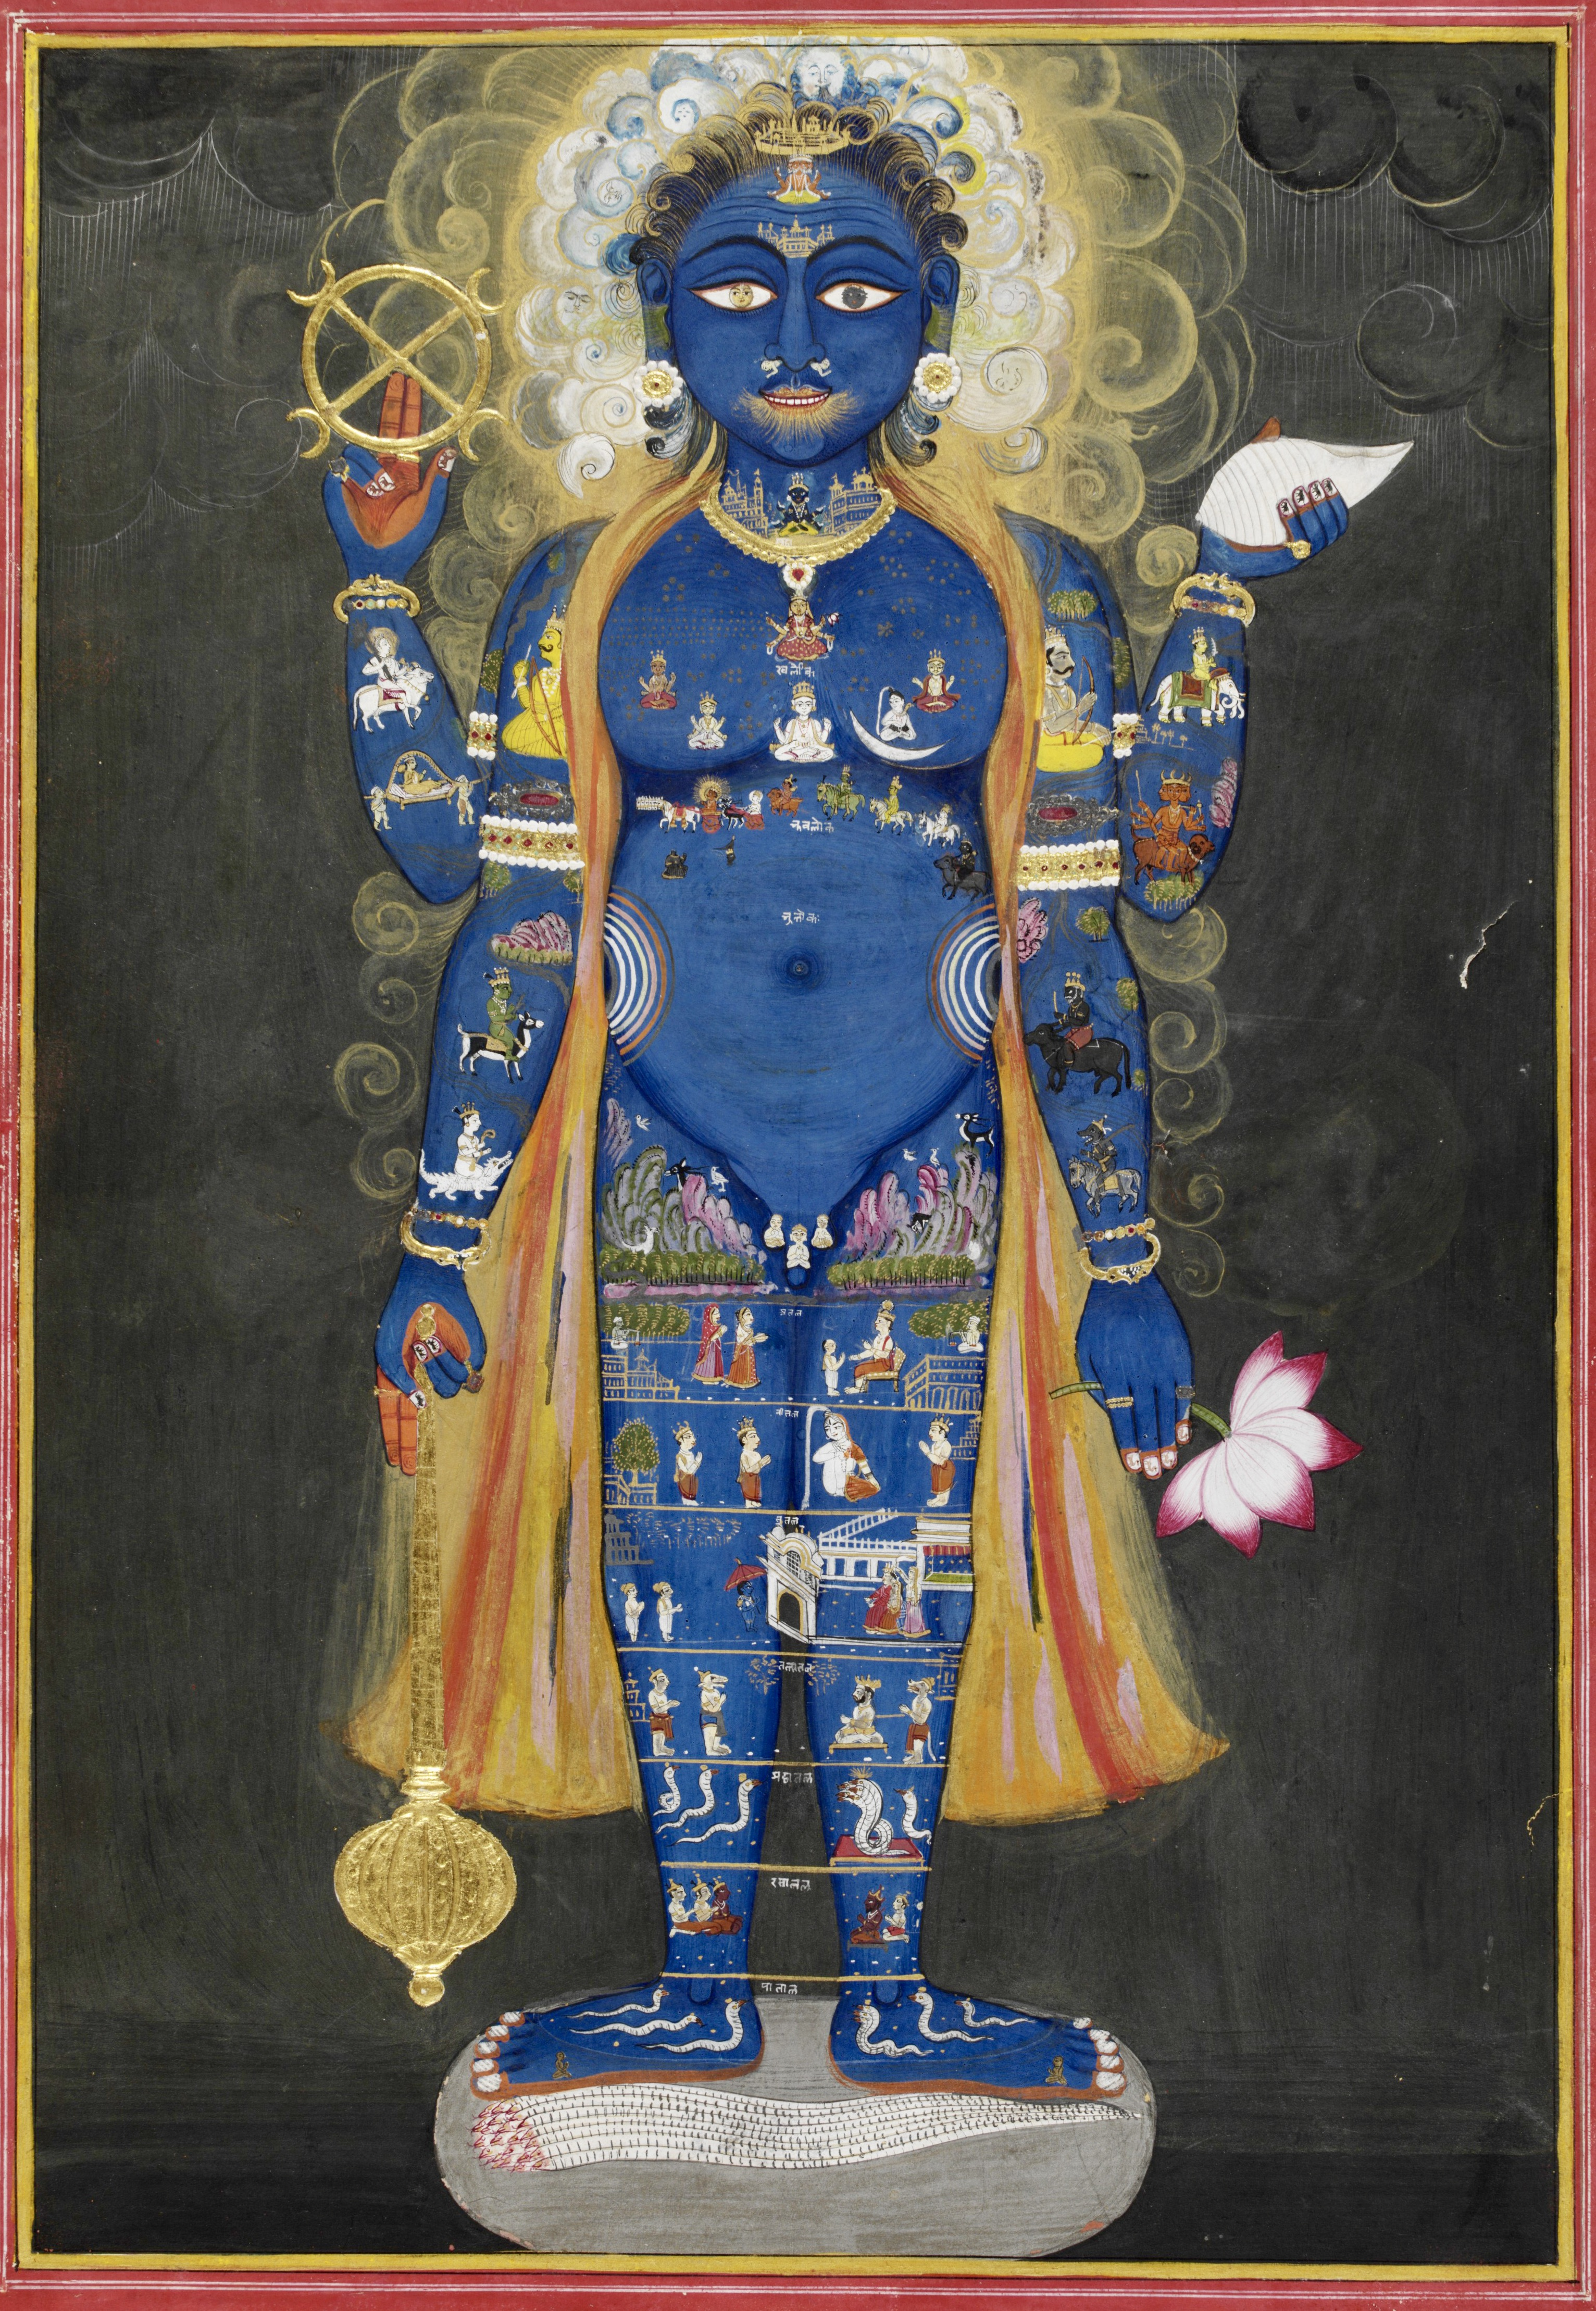
\includegraphics[width=1\textwidth]{pics/Vishnu_Vishvarupa_cropped.jpg}
	\caption{Viṣṇu Viśvarūpa, India, Rajasthan, Jaipur, ca. 1800–1820, Opaque watercolor and gold on paper, 38.5 × 28 cm, Victoria and Albert Museum, London, Given by Mrs. Gerald Clark.}
	\label{fig1}
      \end{figure}
\clearpage
  \begin{figure}[ht]
	\centering
  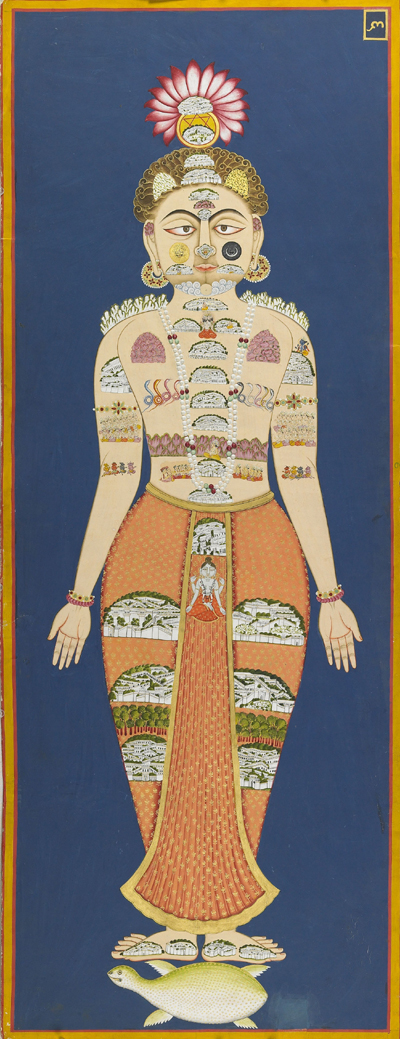
\includegraphics[width=0.5\textwidth]{pics/The_Equivalence_of_Self_and_Universe_(detail),_folio_6_from_the_Siddha_Siddhanta_Paddhati,_(Bulaki),_1824_(Samvat_1881);_122_x_46_cm._Mehrangarh_Museum_Trust..jpg}
	\caption{The Equivalence of Self and Universe (detail), folio 6 from the \textit{Siddhasiddhāntapaddhati} (Bulaki), India, Rajasthan, Jodhpur, 1824 (Samvat 1881), 122 x 46 cm, RJS 2378, Mehragarh Museum Trust.}
	\label{fig2}
      \end{figure}
      % \end{landscape}


\chapter{Bibliography}
 \label{sec:bibli}
   \clearpage
\newpage 
\thispagestyle{empty}
\quad  \addtocounter{page}{-1}

\printbibliography[heading=subbibintoc, title=Consulted Manuscripts, keyword=codex]

\printbibliography[heading=subbibintoc, title=Printed Editions, keyword=printsource]

\printbibliography[heading=subbibintoc, title=Secondary Literature, keyword=seclit]

\printbibliography[heading=subbibintoc, title=Online Sources, keyword=onlinesource]

\end{document}
